\makeatletter
\addtocontents{toc}{\let\protect\l@chapter\protect\l@section}
\addtocontents{toc}{\let\protect\l@section\protect\l@subsection}
\makeatother
\addtocontents{toc}{\protect\setcounter{tocdepth}{1}}
\addtocontents{lof}{\protect\pagebreak}

\chapter{Environments' Details}
\label{sec:environments-details}
The sections of this chapter provide additional details about the custom environments used in our experiments.
Both of these environments were developed in Python.

\section{ShapeGridWorld}
\label{sec:sgw-details}
% Added color
% Added object_persistency 0
% Added step_size > 1
% Improved rendering
% Added partial reset with control and control boundaries
% Added controlled reset with max_dist
% Added partial control with control and control boundaries
\tabref{tab:original-sgw-params} lists the parameters of the original ShapeGridWorld environment developed by \cite{rair}, along with the best values we found for our experiments.
\begin{table}[H]
    \centering
    \caption{Original ShapeGridWorld parameters.}
    \begin{tabularx}{\textwidth}{C{3.9cm} L C{2cm}}
        \hline
        Property & Description & Best/(Default)\\
        \hline
        \texttt{width} & Width of the discrete grid. & \(28\)\\
        \texttt{height} & Height of the discrete grid. Kept same as \texttt{width}. & \(28\)\\
        \texttt{n\_pixels} & Number of ``On'' pixels. & \(\sim 20\)\\
        \texttt{shape} & Shape of a pixel block. & (``circle'')\\
        \texttt{size} & Size of a pixel block. & \(7\)\\
        \texttt{persistency} & Number of time steps an object (pixel block) is moved. & \(1\)\\
        \hline
    \end{tabularx}
    \label{tab:original-sgw-params}
\end{table}
The state space of this environment is composed of the \(x\) and \(y\) coordinates of the \(n\) block pixels, with the addition of two dimensions -- one that specifies which object is currently in focus and another that specifies how many times it has already moved, i.e. \(\cS \in \nN^{2 n + 2}\).
The observation space is a rendering of the grid as an image of shape \(\texttt{width} * \texttt{size} \times \texttt{height} * \texttt{size}\).

The action space comprises the action value for each of the directions (x and y) for an object; \(\cA \in [-1, 1]^{2 n}\).
For each dimension, the controller samples from a continuous distribution in \([-1, 1]\), which is uniformly mapped to \(\{-1, 0, 1\}\) (\([-1, -1/3) \mapsto -1, [-1/3, 1/3] \mapsto 0, (1/3, 1] \mapsto 1\)).

We further added more features to this environment for our experiments, which are listed in \tabref{tab:additional-sgw-params}.
In particular, the ability to move all objects at once and more than one step in an action step was added.
We also developed a controlled reset method with the added feature to freeze sections of the grid, with \texttt{control} and \texttt{control\_boundaries}.
This additionally enabled us to allow the controller only partial access to the environment.
Furthermore, the rendering function was reimplemented using faster methods from \emph{OpenCV}; see \secref{sec:improving-render} for more details.

\begin{table}[H]
    \centering
    \caption{Additional ShapeGridWorld parameters.}
    \begin{tabularx}{\textwidth}{C{3.9cm} L C{2cm}}
        \hline
        Property & Description & Best/(Default)\\
        \hline
        \texttt{step\_x} & Maximum number of steps an object can be translated in the x-direction in one action. & \(7\)\\
        \texttt{step\_y} & Maximum number of steps an object can be translated in the y-direction in one action. Kept same as \texttt{step\_x}. & \(7\)\\
        \texttt{persistency*} & Added the ability to move all objects at once. & \(1\)\\
        \texttt{color} & A flag to enable grayscale values for pixels. & False\\
        \texttt{invert} & A flag to control the inversion of the rendered images.  & True\\
        \texttt{control\_boundaries} & If specified, objects inside these limits \emph{initially} are marked. & (None)\\
        \texttt{control} & A flag to define the scope of control, i.e. whether all the objects or only those marked initially by the control boundaries can be moved. & (``all'')\\
        \texttt{max\_reset\_dist} & Maximum distance an object can be moved from its original position on reset. Only the objects marked initially are reset. There are no constraints if set to \(-1\). & (\(5\))\\
        \hline
    \end{tabularx}
    \label{tab:additional-sgw-params}
\end{table}

If all objects are moved at once, the state space of this environment is composed of only the \(x\) and \(y\) coordinates of the block pixels, i.e. \(\cS \in \nN^{2 n}\).
The corresponding action space in this case would be \(\cA \in [-1, 1]^{2 n}\).
For each dimension of the action space, the controller samples from a continuous distribution in \([-1, 1]\), which is uniformly mapped to integers \([-l, l]\), where \(l \in \{\texttt{step\_x}, \texttt{step\_y}\}\) is the step size of the dimension.

\subsection{ShapeGridWorld Image Registration Technique}
\label{sec:sgw-registration}

To test CLIP inference on ShapeGridWorld and simulate the controller on partial drawings, without having to draw these drawing samples manually, a registration method for images was developed that reads a given image to generate a corresponding ShapeGridWorld of given dimensions.

This is done using a circular convolution kernel over the image to find the corresponding grid pixel values.
Optionally, it makes the lines in the image thinner by finding its skeleton using morphological operations before the convolution.
See \figref{fig:sgw-registration} for a demonstration.

% \vspace{12pt}
\begin{figure}[H]
    \centering
    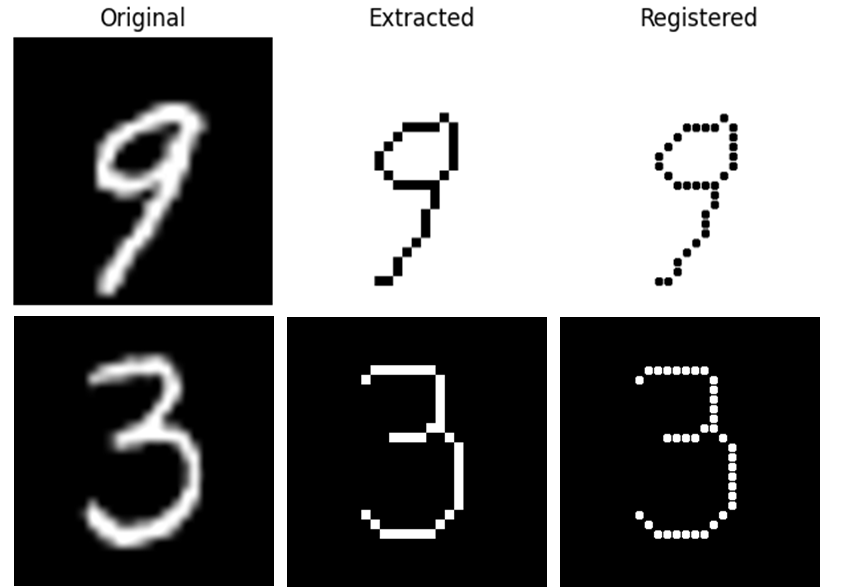
\includegraphics[width=0.66\textwidth]{images/grid_registration.png}
    \caption{ShapeGridWorld image registration on images from the MNIST dataset.}
    \label{fig:sgw-registration}
\end{figure}
% \vspace{12pt}

We developed a wrapper around the PIL Python library \citep{pil} to conveniently perform these operations and generate ShapeGridWorld environments.
The relevant code is hosted on \url{https://github.com/pulkitgoyal56/ImageGrid}.
\tabref{tab:imagelib-params} lists the relevant parameters of this image registration library, along with the default values.
\begin{table}[H]
    \centering
    \caption{Image registration parameters.}
    \begin{tabularx}{\textwidth}{C{3.9cm} L C{2cm}}
        \hline
        Property & Description & Default\\
        \hline
        \texttt{mode} & PIL Image mode in which the image is read. & ``1'' (Binary)\\
        \texttt{invert} & A flag to control the inversion of the read image. The expected image should be white on black. & False \\
        \texttt{threshold\_ratio} & Threshold on the convolution sum, for binary grids. & \(0\)\\
        \hline
    \end{tabularx}
    \label{tab:imagelib-params}
\end{table}

\section{Tangram}
\label{sec:tangram-details}
% flip
% rotate
% x_size
% r_size
% x_step
% object_persistency
% max_dist
% control
% control_boundaries
% staging_boundaries

The Tangram environment is constructed with a list of polygon objects created using the provided \texttt{Polygon} class, which defines a polygon's size, shape, and color.
The additional parameters of the Tangram environment are tabulated in table \tabref{tab:tangram-params}.
\begin{table}[H]
    \centering
    \caption{Tangram parameters.}
    \begin{tabularx}{\textwidth}{C{3.9cm} L C{2cm}}
        \hline
        Property & Description & Best/(Default)\\
        \hline
        \texttt{x\_size, y\_size} & Span of the discrete grid; number of steps in the x and y directions. If set to \(1\), grid is continuous in \([0, 1]\). & \(1\)\\
        \texttt{x\_step, y\_step} & Maximum number of steps a polygon can be translated in the x and y directions in one action. & \(5\)\\
        \texttt{r\_size} & Span of the discrete grid; number of rotation steps in \(180^\circ\). If set to \(1\), rotation is continuous in \([0, 180^\circ]\). & \(1\)\\
        \texttt{r\_step} & Maximum number of steps a polygon can be rotated in one action. & \(4\)\\
        \texttt{rotate} & A flag to enable/disable rotation. & True\\
        \texttt{flip} & A flag to enable/disable flipping. & False\\
        \texttt{persistency} & Number of time steps a polygon (pixel block) is moved. If set to \(1\), all polygons are moved at once. & \(1\)\\
        \texttt{control\_boundaries} & If specified, polygons inside these limits \emph{initially} are marked. & (None)\\
        \texttt{control\_criteria} & The point inside the polygon that determines if the polygon is inside or outside the control boundaries. A Python lambda function or an attribute of \texttt{Polygon}, such as ``centroid'' for the centroid, ``center'' for the mean of the vertices, or ``complete'' for the entire polygon. & (``center'')\\
        \texttt{control} & A flag to define the scope of control, i.e. whether all the polygons or only those marked initially by the control boundaries can be moved. & (``all'')\\
        \texttt{staging\_boundaries} & If specified, only polygons inside these limits are rendered to get a state's corresponding image observation. See \figref{fig:staging-boundaries} & None\\
        \texttt{staging\_criteria} & Like \texttt{control\_criteria} but for staging boundaries. & (``complete'')\\
        \texttt{max\_reset\_dist} & Maximum distance a polygon can be moved from its original position on reset. Only the polygons marked initially are reset. There are no constraints if set to \(-1\). & (\(-1\))\\
        \hline
    \end{tabularx}
    \label{tab:tangram-params}
\end{table}

% staging_crop.png
% staging_crop_color.png
% staging_nocrop.png
% staging_nocrop_color.png
\begin{figure}[h]
    \centering
    % \subfloat{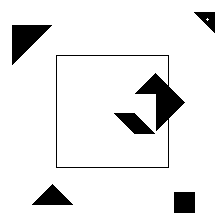
\includegraphics[width=0.2\textwidth]{images/staging_nocrop.png}}
    % \subfloat{
\includegraphics[width=0.2\textwidth]{images/staging_crop.png}}
    % \subfloat{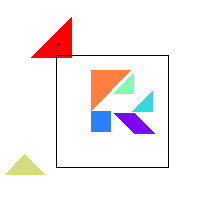
\includegraphics[width=0.2\textwidth]{images/staging_nocrop_color.png}}
    % \subfloat{
\includegraphics[width=0.2\textwidth]{images/staging_crop_color.png}}
    \subfloat{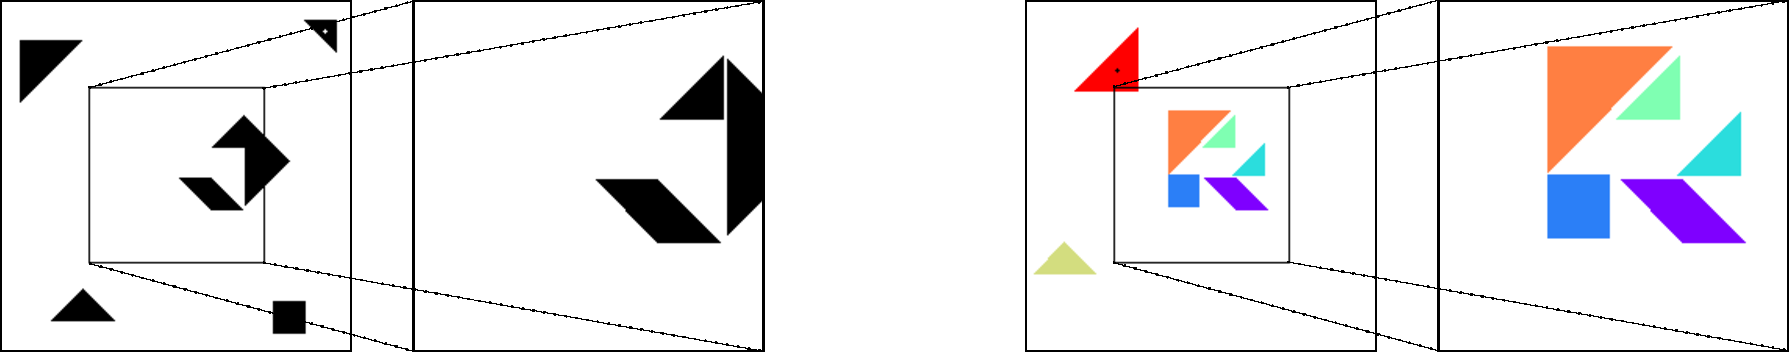
\includegraphics[width=\textwidth]{images/staging_boundaries.pdf}}
    \caption[Staging boundaries in the Tangram environment.]{Staging boundaries in the Tangram environment. Simulations using staging boundaries can be viewed at \url{https://drive.google.com/drive/u/0/folders/1PLopyNdzpWiz6CK4EvR8oEAScACpUsW0}.}
    \label{fig:staging-boundaries}
\end{figure}

The state space of this environment is composed of the \(x\) and \(y\) coordinates of the vertices of the \(n = 7\) polygons, with the addition of two dimensions -- one that specifies which polygon is currently in focus and another that specifies how many times it has already moved, i.e. \(\cS \in \nN^{\,2 + \sum_{i \in n} 2\ n_v(p_i)}\), where \(n_v(p_i)\) is the number of vertices of polygon \(p_i\).
If all polygons are moved at once, the state space of this environment is composed of only the \(x\) and \(y\) coordinates of the block pixels, i.e. \(\cS \in \nN^{\sum_{i \in n} 2\ n_v(p_i)}\).
The observation space is a rendering of the grid whose resolution is controlled with different parameters.

The action space comprises the action value for each of the degrees of freedom (x, y, rotation, and flip) for an object; \(\cA \in [-1, 1]^4\).
For each dimension of the action space, the controller samples from a continuous distribution in \([-1, 1]\).
In the x-, y-, and rotation dimensions, this is uniformly mapped to integers in \([-l, l]\), where \(l \in \{\texttt{step\_x}, \texttt{step\_y}, \texttt{step\_r}\}\) is the step size of the dimension, if it is discrete.
If the dimension is continuous (because its \texttt{size} is set to \(1\)), the action is scaled by its respective step size instead.
The \texttt{step} parameter can then be understood as the minimum number of actions required to move a polygon across the entire grid.
For example, if \texttt{x\_size} is \(1\) and \texttt{x\_step} is \(3\), the resulting support of the action distribution for any action sampled for x-dimension will be \([-1/3, 1/3]\).
For the flip dimension, the mapping is (\([-1, 0] \mapsto \texttt{False}, (0, 1] \mapsto \texttt{True}\)).

The developed code to create Tangram-like environments with any number of arbitrary convex polygons is available on \url{https://github.com/pulkitgoyal56/Tangram}.

\chapter{Controller Hyperparameters}
\label{sec:icem-details}
% task_horizon
% horizon
% num_simulated_trajectories
% cost_along_trajectory
% action_sampler_params.opt_iterations
% action_sampler_params.init_std
% action_sampler_params.elites_size
% discount_along_trajectory
The iCEM controller introduced in \secref{sec:icem} has several hyperparameters that need to be tuned for optimal performance.
\tabref{tab:icem-params} lists the hyperparameters we tweaked in our experiments, along with the best values we found.

\begin{table}[H]
    \centering
    \caption{iCEM controller parameters.}
    \begin{tabularx}{\textwidth}{C{4.7cm} L C{2cm}}
        \hline
        Property & Description & Best\\
        \hline
        \texttt{horizon} & Number of steps in the future to plan, \(h\) & \(16\).\\
        \texttt{n\_trajectories} & Number of trajectories to sample, \(n\). & \(128\)\\
        \texttt{cost\_along\_trajectory} & Cost/reward aggregation function to evaluate the trajectory, \(g\). See \secref{sec:reward-aggregation} for explanations. & \texttt{best} or \texttt{sum}\\
        \texttt{n\_inner\_iterations} & Number of iterations for the inner optimization loop, \(m\). & \(3\)\\
        \texttt{init\_std} & Standard deviation at which the sampling distribution is initialized, \(\bmsigma_0\). & \(0.6\)\\
        \texttt{elites\_size} & Size of the elite set, \(K\). See eq. \eqref{eq:icem-filter}. & \(20\)\\
        \texttt{discount\_factor} & Discount factor for returns expected in the future, \(\gamma\). See eq. \eqref{eq:reward-aggregation-sum-discount}. & \(1.0\)\\ 
        \hline
    \end{tabularx}
    \label{tab:icem-params}
\end{table}

The other important hyperparameters that we did not tweak in our experiments are listed in \tabref{tab:icem-params-fixed}.

% factor_decrease_num: 1
% alpha: 0.1
% relative_init: true
% keep_previous_elites: true
% shift_elites_over_time: true
% fraction_elites_reused: 0.3
% use_mean_actions: true
% noise_beta: 3.5

\begin{table}[H]
    \centering
    \caption{iCEM controller fixed parameters.}
    \begin{tabularx}{\textwidth}{C{4.7cm} L C{2cm}}
        \hline
        Property & Description & Default\\
        \hline
        \texttt{factor\_decrease\_num} & Factor by which population size is decreased. & \(1.0\)\\
        \texttt{alpha} & Momentum term for updating parameters of the sampling distribution. & \(0.1\)\\
        % \texttt{relative\_init} & \\
        \texttt{keep\_previous\_elites} & A flag to enable passing elites to the next timestamp (outer iteration). & True\\
        \texttt{shift\_elites\_over\_time} & A flag to enable passing elites over inner iterations. & True\\
        \texttt{fraction\_elites\_reused} & Fraction of passed elites from the previous iteration (inner/outer) added to the sampled trajectory set. & \(0.3\)\\
        \texttt{use\_mean\_actions} & If the mean of the sampling distribution is appended to the elite set at the end of inner iterations. & True\\
        \texttt{noise\_beta} & Colored noise exponent of the distribution, \(\beta\) & \(1.0\).\\
        \hline
    \end{tabularx}
    \label{tab:icem-params-fixed}
\end{table}

Please refer to the original paper for more details on the parameters of iCEM.

\chapter{Reward Hyperparameters}
\label{sec:reward-details}

This chapter details the hyperparameters of the reward functions used in our experiments.

\section{Semantics Reward}
\label{sec:semantics-reward-details}

\subsection{Semantics Entropy Reward}
\label{sec:semantics-entropy-reward-details}
% label_prefix
% label_suffix
% categories
% semantics_baseline
% semantics_image_baseline
% semantics_alpha_target
% semantics_beta_image
% semantics_model_temperature
% semantics_model_version
% semantics_normalize
% semantics_reward_scale

\tabref{tab:entropy-reward-params} lists the parameters of the regularized semantics entropy reward from eq. \eqref{eq:entropy-reward-reg}, along with the best values we found for our experiments.
\begin{table}[H]
    \centering
    \caption{Semantics entropy reward parameters.}
    \begin{tabularx}{\textwidth}{C{3.9cm} L C{2cm}}
        \hline
        Property & Description & Best\\
        \hline
        \texttt{categories} & List of creative possibilities, \(\bml\). & \(|l| \approx 20\)\\
        \texttt{label\_prefix} & Prefix to be added to the categories to create text labels.\\
        \texttt{label\_suffix} & Suffix to be added to the categories to create text labels.\\
        \texttt{baseline} & Baseline text input, \(\bfl_b\). ``A white canvas''\\
        \texttt{image\_baseline} & Baseline image input, \(\bfi_b\).\\
        \texttt{alpha\_target} & Regularization parameter for target text, \(\alpha\). & \(0.5\)\footnotemark[1]\\
        \texttt{beta\_image} & Regularization parameter for input image observation, \(\beta\). & \(0\)\footnotemark[1]\\
        \texttt{model\_version} & Name of the CLIP variant used. & (\texttt{ViT-L/14})\\
        \texttt{model\_temperature} & Temperature for the softmax function in the semantics entropy reward, \(T\). & \([1, 2]\)\\
        \texttt{normalize} & If the reward should be normalized by maximum entropy, \(\log(|\bml|)\). & True\\
        \texttt{reward\_scale} & Factor with which the reward is scaled. Together with the \texttt{reward\_scale} for the regularity reward, this determines the reward ratio, \(\lambda\) from eq. \eqref{eq:semantics-reward}. & \(1.0\)\\
        \hline
    \end{tabularx}
    \label{tab:entropy-reward-params}
\end{table}
\footnotetext[1]{Please see \secref{sec:alpha-beta-semantics} for more details.}

\newpage
\subsection{Regularity Reward}
\label{sec:regularity-reward-details}
% compression_precision
% compression_granularity
% compression_bidirectional
% compression_normalize
% compression_reward_scale

In the introduction to the regularity reward in \secref{sec:regularity-reward}, we mentioned the additional hyperparameters \(h\) -- \emph{resolution} and \emph{bidirectionality}.
This section provides more details about these hyperparameters.

The hyperparameter for resolution consists of two parts -- precision and granularity.
Equation \eqref{eq:rair-relational-extended} extends eq. \eqref{eq:rair-relational} with these hyperparameters to define the \(\lfloor \cdot \rceil\) operator.
\begin{equation}
    \lfloor s^{(j)} - s^{(k)} \rceil = \begin{cases}\begin{aligned}
        \left\lfloor \left| s^{(j)} - s^{(k)} \right| \frac{\text{precision}}{\text{granularity}} \right\rfloor \times \text{granularity},\quad&\text{if bidirectionality} = \text{False}\\
        \left\lfloor \left( s^{(j)} - s^{(k)} \right) \frac{\text{precision}}{\text{granularity}} \right\rfloor \times \text{granularity},\quad&\text{if bidirectionality} = \text{True}\\
    \end{aligned}\end{cases}
    \label{eq:rair-relational-extended}
\end{equation}
\tabref{tab:regularity-reward-params} lists the parameters of the regularity reward, along with the (default or) best values we found for our experiments.
\begin{table}[H]
    \centering
    \caption{Regularity reward parameters.}
    \begin{tabularx}{\textwidth}{C{3.9cm} L C{2cm}}
        \hline
        Property & Description & Best\\
        \hline
        \texttt{precision} & Precision of the compression algorithm. Equal to the grid size for discrete grids. & SGW - \(28\) Tangram - \(1\)\\
        \texttt{granularity} & Granularity of the compression algorithm. & \(1\)\\
        \texttt{bidirectional} & If the compression should be bidirectional. & False\\
        \texttt{normalize} & If the reward should be normalized by the maximum possible entropy, \(\log\left(\binom{N}{2}\right)\). & True\\
        \texttt{reward\_scale} & Factor with which the reward is scaled. Together with the \texttt{reward\_scale} for the semantics entropy reward, this determines the reward ratio, \(\lambda\) from eq. \eqref{eq:semantics-reward}. & \(1.0\)\\
        \hline
    \end{tabularx}
    \label{tab:regularity-reward-params}
\end{table}

Please refer to the original paper for more details on the theory and implementation of \emph{RaIR}.

\section{Closeness Reward}
\label{sec:closeness-reward-details}
% closeness_reward_type
% closeness_reward_scale
% closeness_reward_threshold

\tabref{tab:closeness-reward-params} lists the parameters of the closeness reward from \secref{sec:closeness-rollouts}.
\begin{table}[H]
    \centering
    \caption{Closeness reward parameters.}
    \begin{tabularx}{\textwidth}{C{3.9cm} L C{2cm}}
        \hline
        Property & Description & Default\\
        \hline
        \texttt{reward\_type} & Type of closeness reward -- \emph{sparse-incremental} or \emph{dense}. & ``sparse''\\
        \texttt{reward\_scale} & Factor with which the reward is scaled. & \(1.0\)\\
        \texttt{reward\_threshold} & Threshold, \(\varepsilon\), for sparse rewards, eq. \eqref{eq:closeness-reward-sparse}. & \(0.051\)\\
        \hline
    \end{tabularx}
    \label{tab:closeness-reward-params}
\end{table}

% - controller_params.compression                           True
% - controller_params.render_kwargs.invert                  True
% - controller_params.render_kwargs.color                   False
% - controller_params.semantics_baseline                    "A white canvas"
% - controller_params.action_sampler_params.opt_iterations  3
% - controller_params.action_sampler_params.init_std        0.6
% - controller_params.action_sampler_params.elites_size     20
% - controller_params.num_simulated_trajectories            256
% - controller_params.horizon                               8
% - env_params.x_size                                       28
% - env_params.x_step                                       7
% - controller_params.compression_precision                 28
% - env_params.staging_boundaries                           `[[0.25, 0.25], [0.75, 0.75]]`
% - env_params.object_persistency                           0
% - controller_params.semantics_model_temperature           1
% - controller_params.semantics_alpha_target                0.5
% - controller_params.semantics_beta_image                  0
% - controller_params.semantics_reward_scale                1
% - controller_params.cost_along_trajectory                 "best"

\chapter{Comparing CLIP Models}
\label{sec:clip-comparison}

The vision transformer (ViT) models have better accuracy than Resnet models.
Resnet models have a gradual slope in rollouts compared to ViT models and flatter distributions on random images.

\begin{figure}[H]
    \centering
    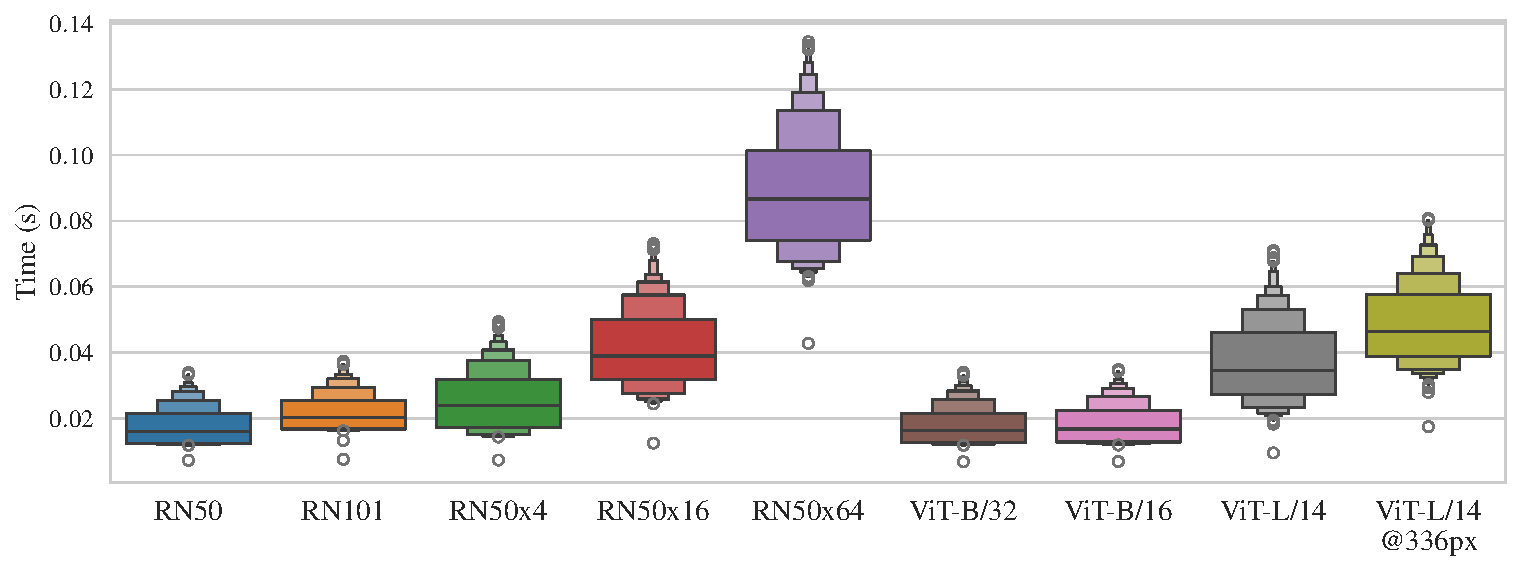
\includegraphics[width=\textwidth]{images/clip_inference_times.pdf}
    \vspace{-12pt}
    \caption{Comparing times of different original CLIP models for embedding a single image.}
    \label{fig:clip-time-comparison}
\end{figure}

\figref{fig:clip-traj-comparison-color} shows the trajectories of different CLIP models on colored Tangram environments (without RaIR).
The cumulative rewards and trajectories of the models are similar and do not give a clear picture of the models' performances, but the larger models seem to have better creations. 

% \begin{figure}[H]
%     \centering
%     % model_comparison.pdf
%     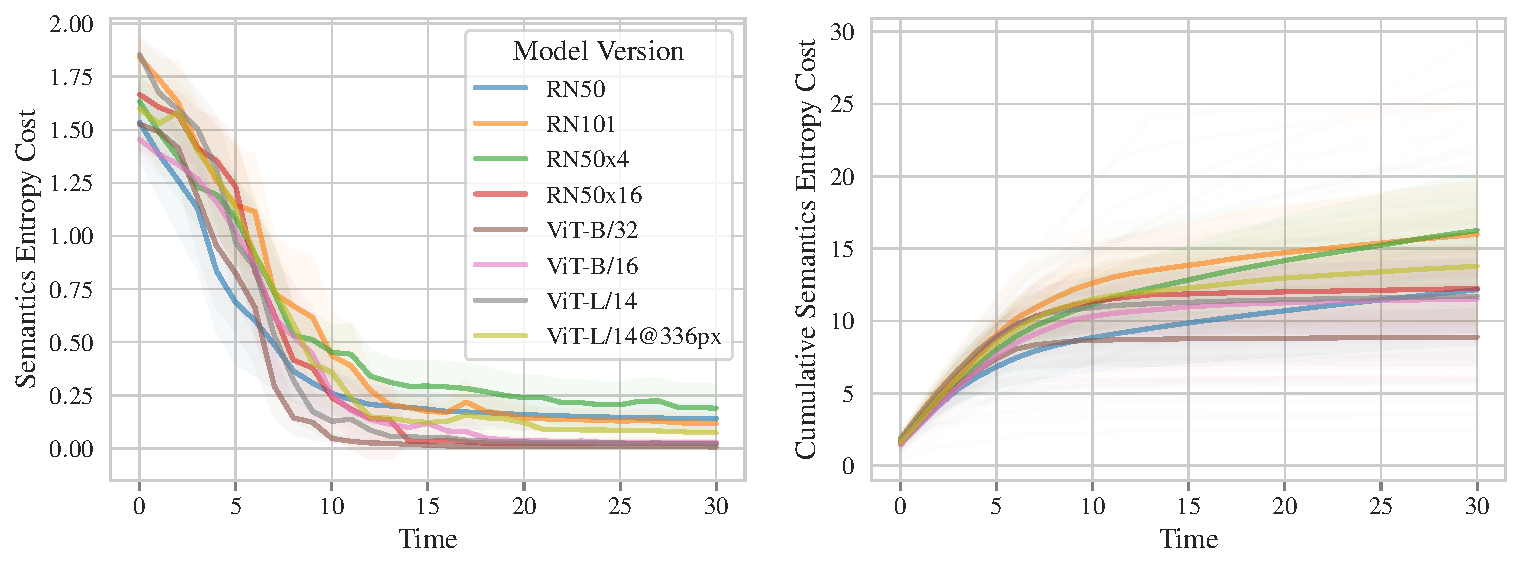
\includegraphics[width=\textwidth]{images/model_comparison.pdf}
%     % model_comparison_boxplot.pdf
%     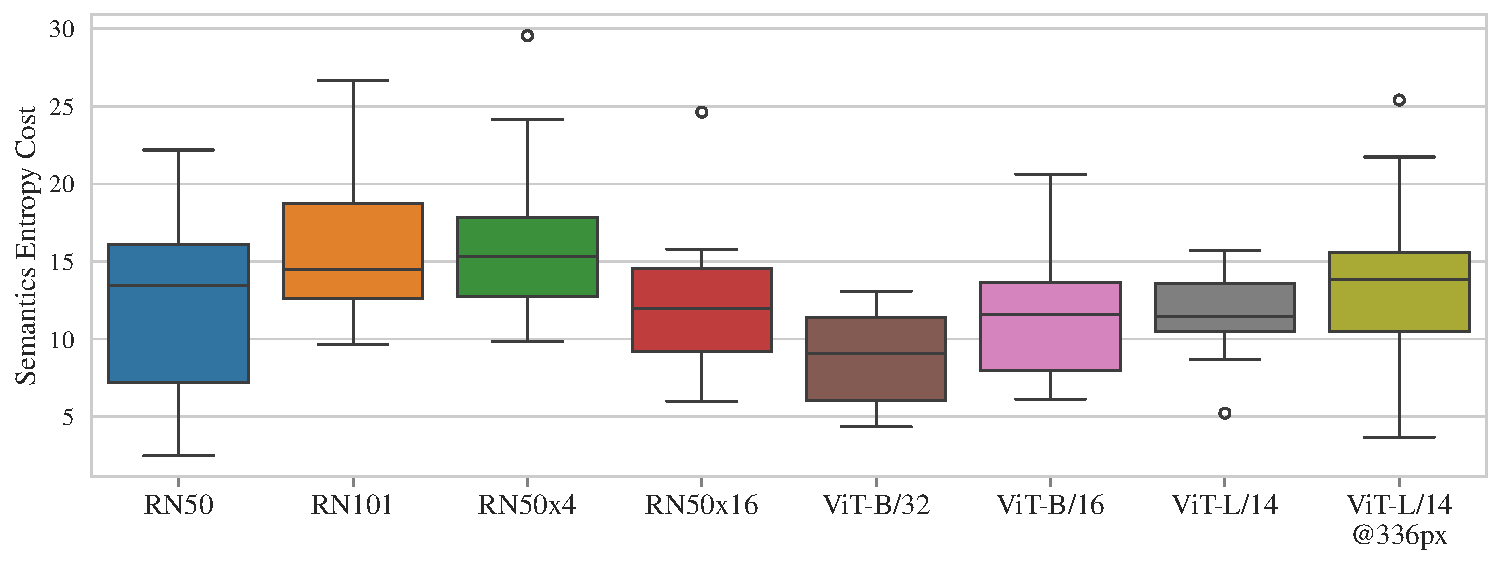
\includegraphics[width=\textwidth]{images/model_comparison_boxplot.pdf}
%     % model_samples.pdf
%     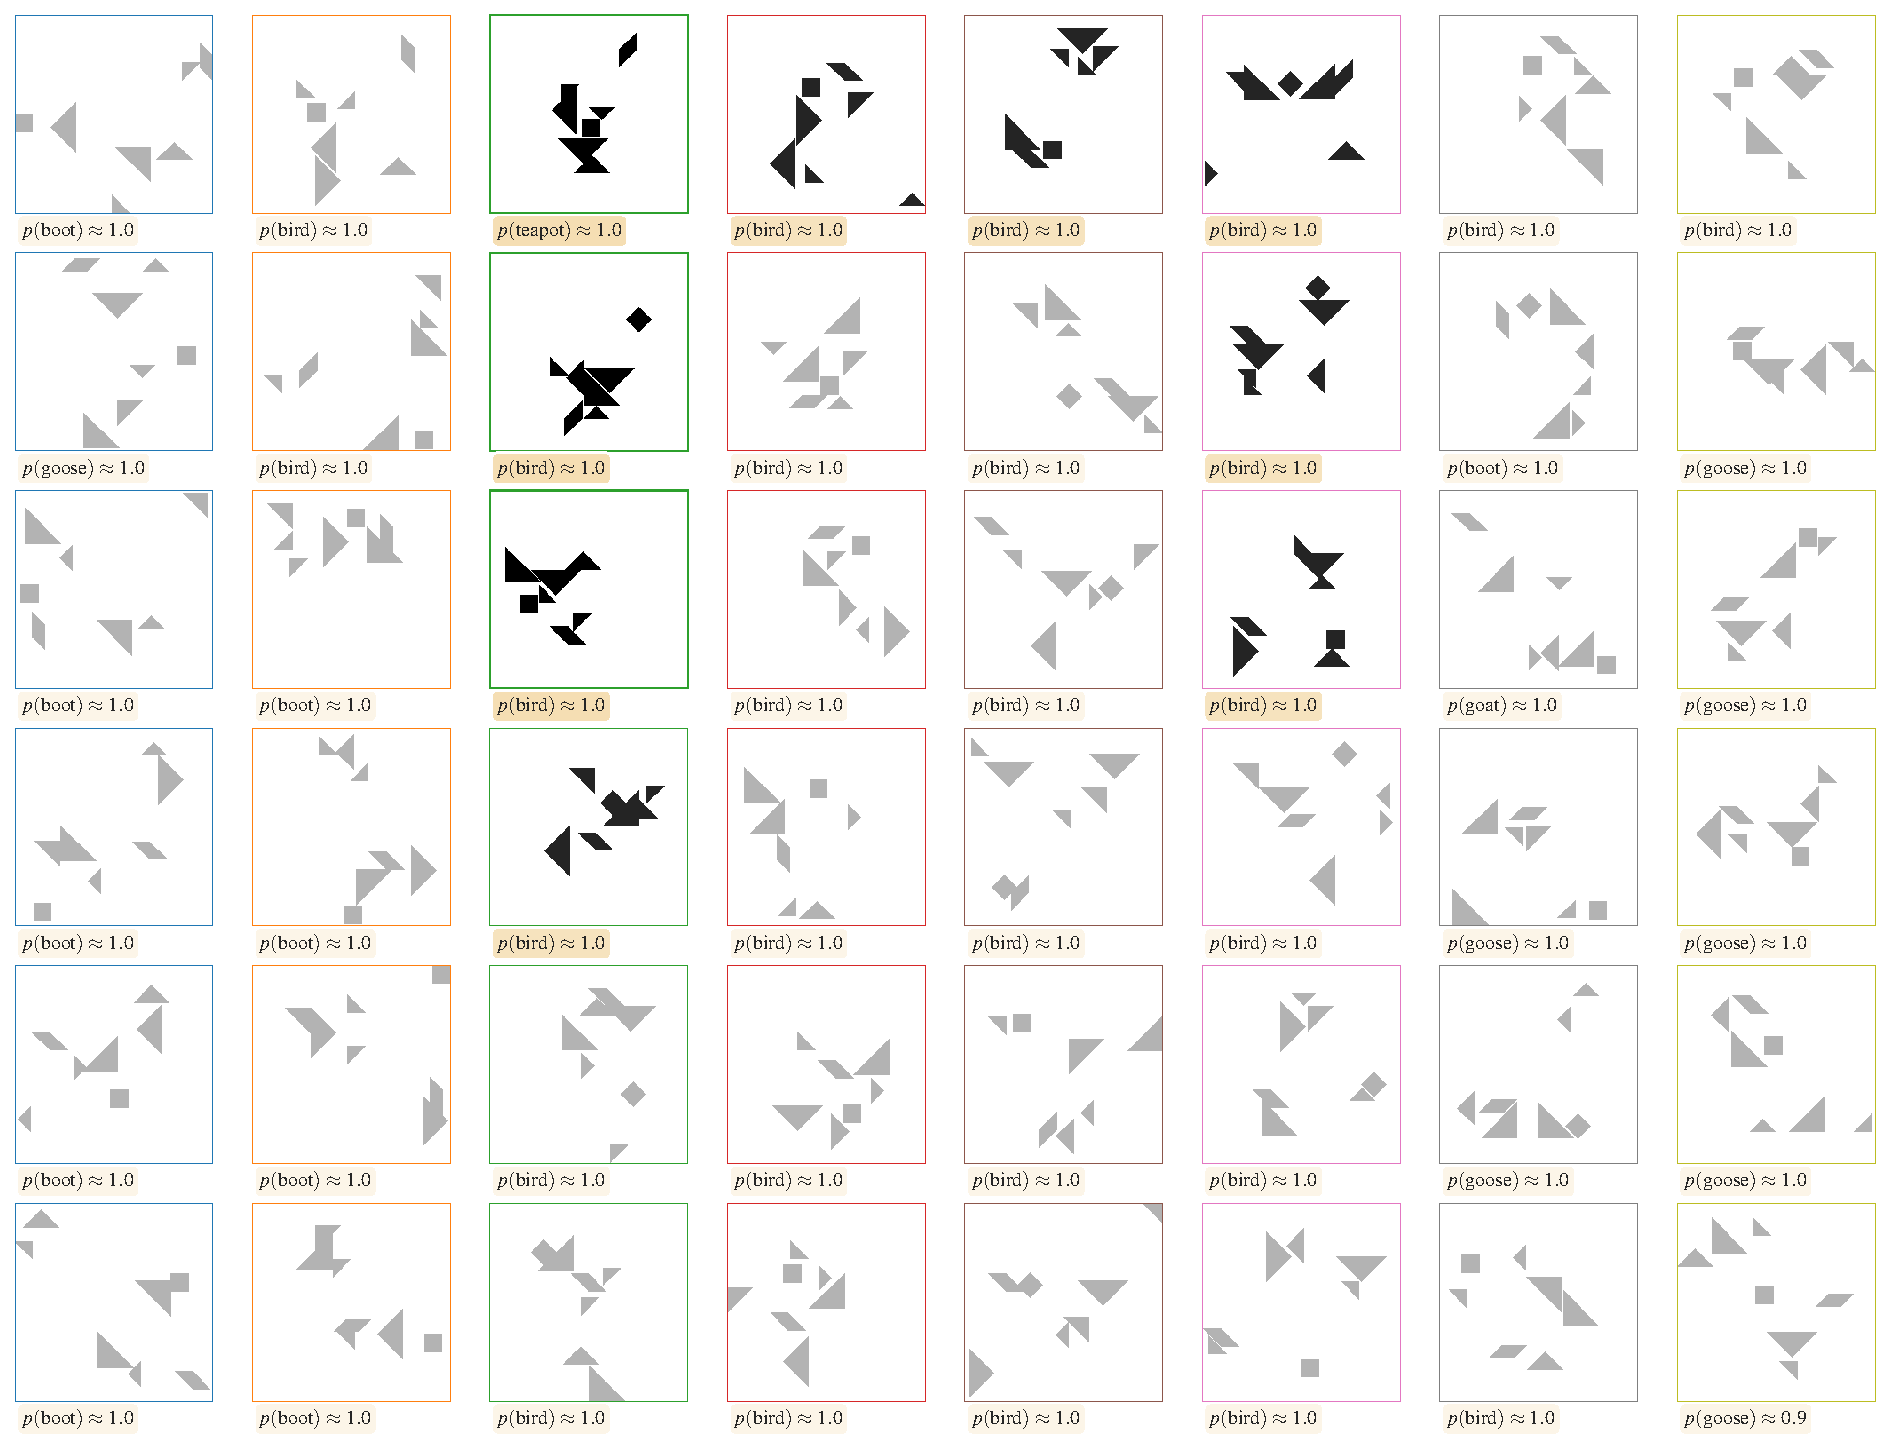
\includegraphics[width=0.9\textwidth]{images/model_samples.pdf}
%     \caption[Comparing reward trajectories of different original CLIP models on b/w Tangram environment.]{Comparing reward trajectories of different original CLIP models on b/w Tangram environment. 10 seeds were used for each model.}
%     \label{fig:clip-traj-comparison}
% \end{figure}

\begin{figure}[H]
    \centering    
    % model_comparison_color.pdf
    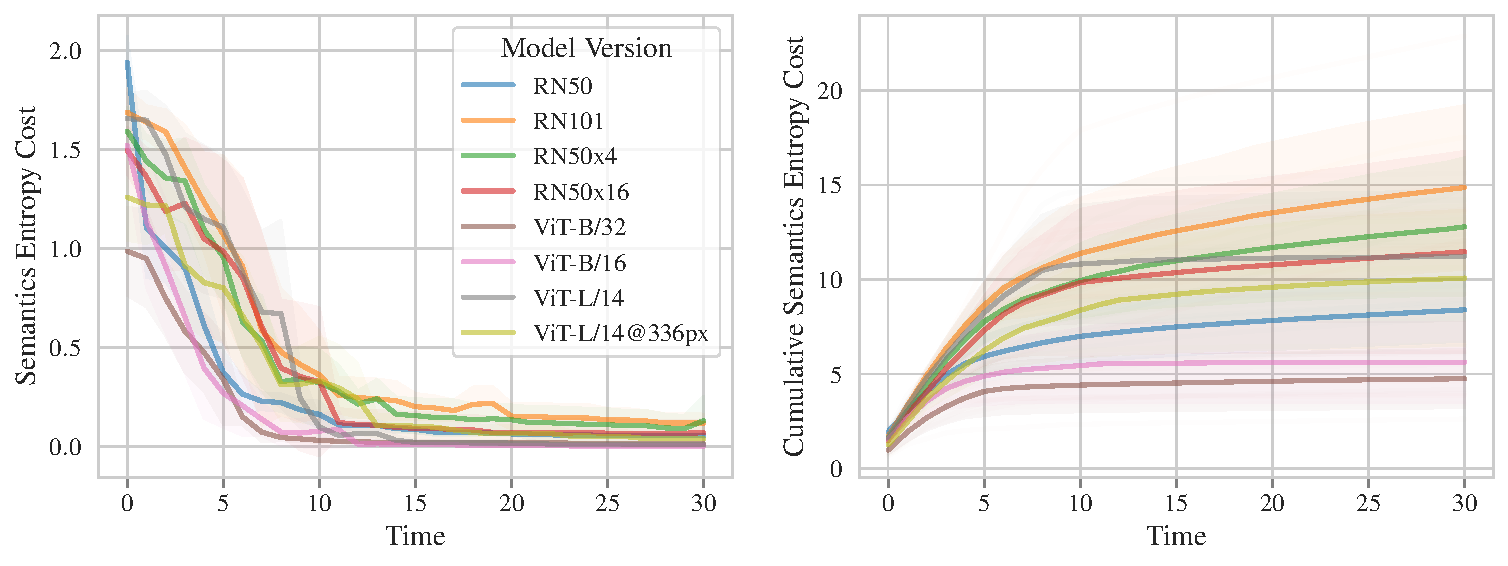
\includegraphics[width=\textwidth]{images/model_comparison_color.pdf}
    % model_comparison_boxplot_color.pdf
    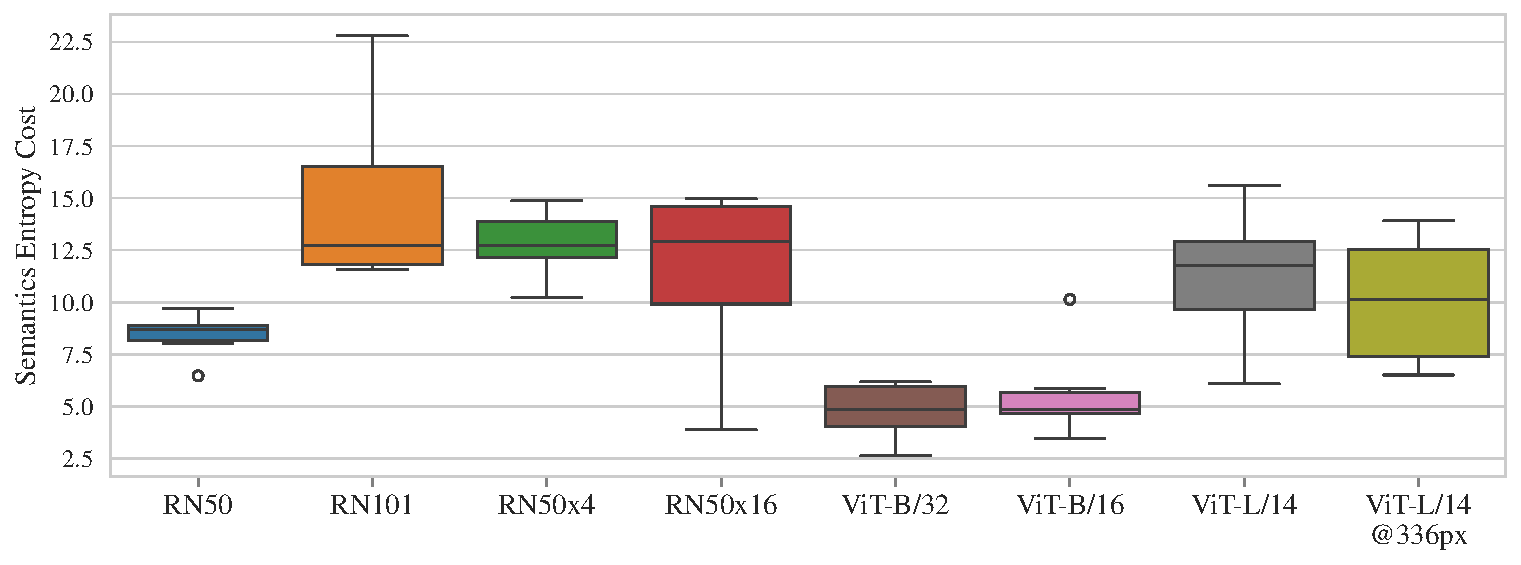
\includegraphics[width=\textwidth]{images/model_comparison_boxplot_color.pdf}
    % model_samples_color.pdf
    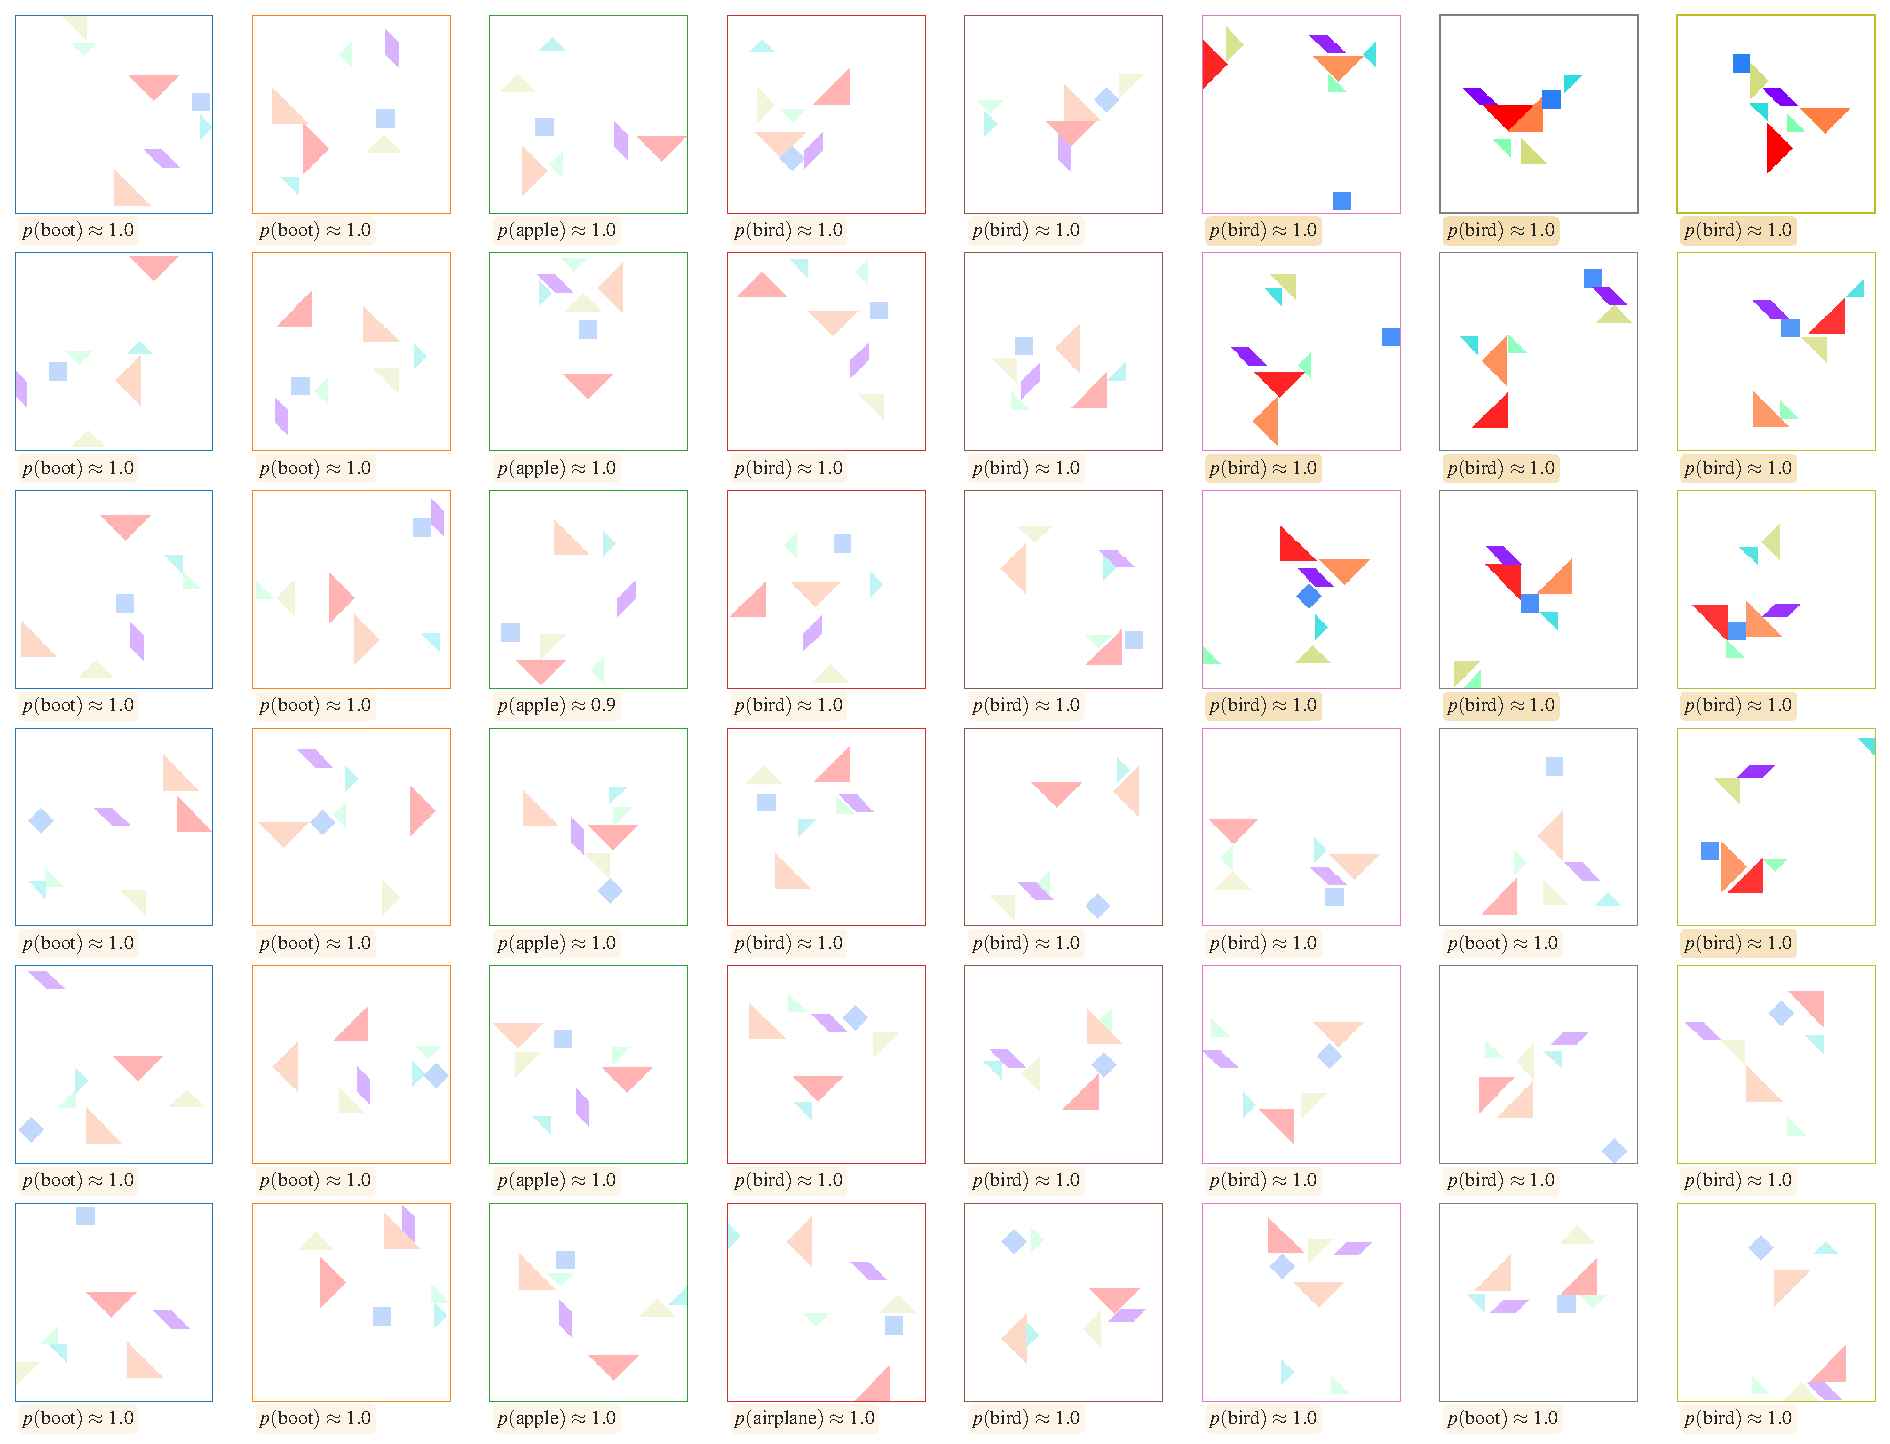
\includegraphics[width=0.9\textwidth]{images/model_samples_color.pdf}
    \caption[Comparing reward trajectories of different original CLIP models on colored Tangram environment.]{Comparing reward trajectories of different original CLIP models on colored Tangram environment. 10 seeds were used for each model.}
    \label{fig:clip-traj-comparison-color}
\end{figure}


\chapter{Flatnet}
\label{sec:flatnet}
To test the feasibility and efficacy of fine-tuning CLIP with an entropy regularization technique (eq. \ref{eq:entropy-regularization}) to reduce its inference noise, we conducted experiments on a smaller \emph{toy} setup with convolutional neural networks trained as a single-digit number classifier on ShapeGridWorld registered images from the MNIST dataset \citep{mnist}.
We additionally augmented the MNIST training dataset with samples of images with random arrangements of pixels, target-labeled with a uniform distribution of confidence over the ten single digits.

We treated the entropy regularization strength and the addition of random samples as hyperparameters and trained a series of models with different combinations of the two.
% \figref{fig:flatnet-comparison} shows the resulting trajectories of the models.
The models were trained with the Adam optimizer \citep{adam} with a learning rate of \(0.001\) and a batch size of \(128\). The size of the MNIST training dataset is \(60000\).
\tabref{tab:flatnet-models} summarizes the models we trained.
More details of these models can be found at \url{https://pulkitgoyal56.github.io/flatnet}.

% \vspace{12pt}
\begin{table}[H]
    \centering
    \caption{Summary of the Flatnet models.}
    \begin{tabularx}{0.7\textwidth}{c c c c}
    \hline
        Serial & Name & Random Training Data Size & \(\lambda\) \\ \hline
        Flatnet 0 (lite) & flatnetlite & 0 & 0.0 \\ \hline
        Flatnet 1 (lite) & flatnetlite & 0 & 0.2 \\ \hline
        Flatnet 2 & flatnet & 0 & 0.2 \\ \hline
        Flatnet 3 & flatnet & 0 & 0.4 \\ \hline
        Flatnet 4 & flatnet & 0 & 0.6 \\ \hline
        Flatnet 5 & flatnet & 0 & 0.8 \\ \hline
        Flatnet 6 & flatnet & 0 & 1.0 \\ \hline
        Flatnet 7 & flatnet & 10000 & 0.0 \\ \hline
        Flatnet 8 & flatnet & 10000 & 0.3 \\ \hline
        Flatnet 9 & flatnet & 10000 & 0.7 \\ \hline
        Flatnet 10 & flatnet & 10000 & 0.8 \\ \hline
        Flatnet 11 & flatnet & 10000 & 1.0 \\ \hline
        Flatnet 12 & flatnet & 0 & 1.0 \\ \hline
        Flatnet 13 & flatnet & 60000 & 0.0 \\ \hline
        Flatnet 15 & flatnet & 0 & 0.0 \\ \hline
    \end{tabularx}
    \label{tab:flatnet-models}
\end{table}

\figref{fig:flatnet-comparison} compares the reward trajectories of a regular Flatnet model and an entropy regularized Flatnet model on random rollouts (similar to \figref{fig:sparse-rewards}) on a grid-registered image of the number zero.
The comparisons of all the models are neatly visualized at \url{https://www.sharecanvas.io/p/flatnet-comparison}.

\begin{figure}[H]
    \centering
    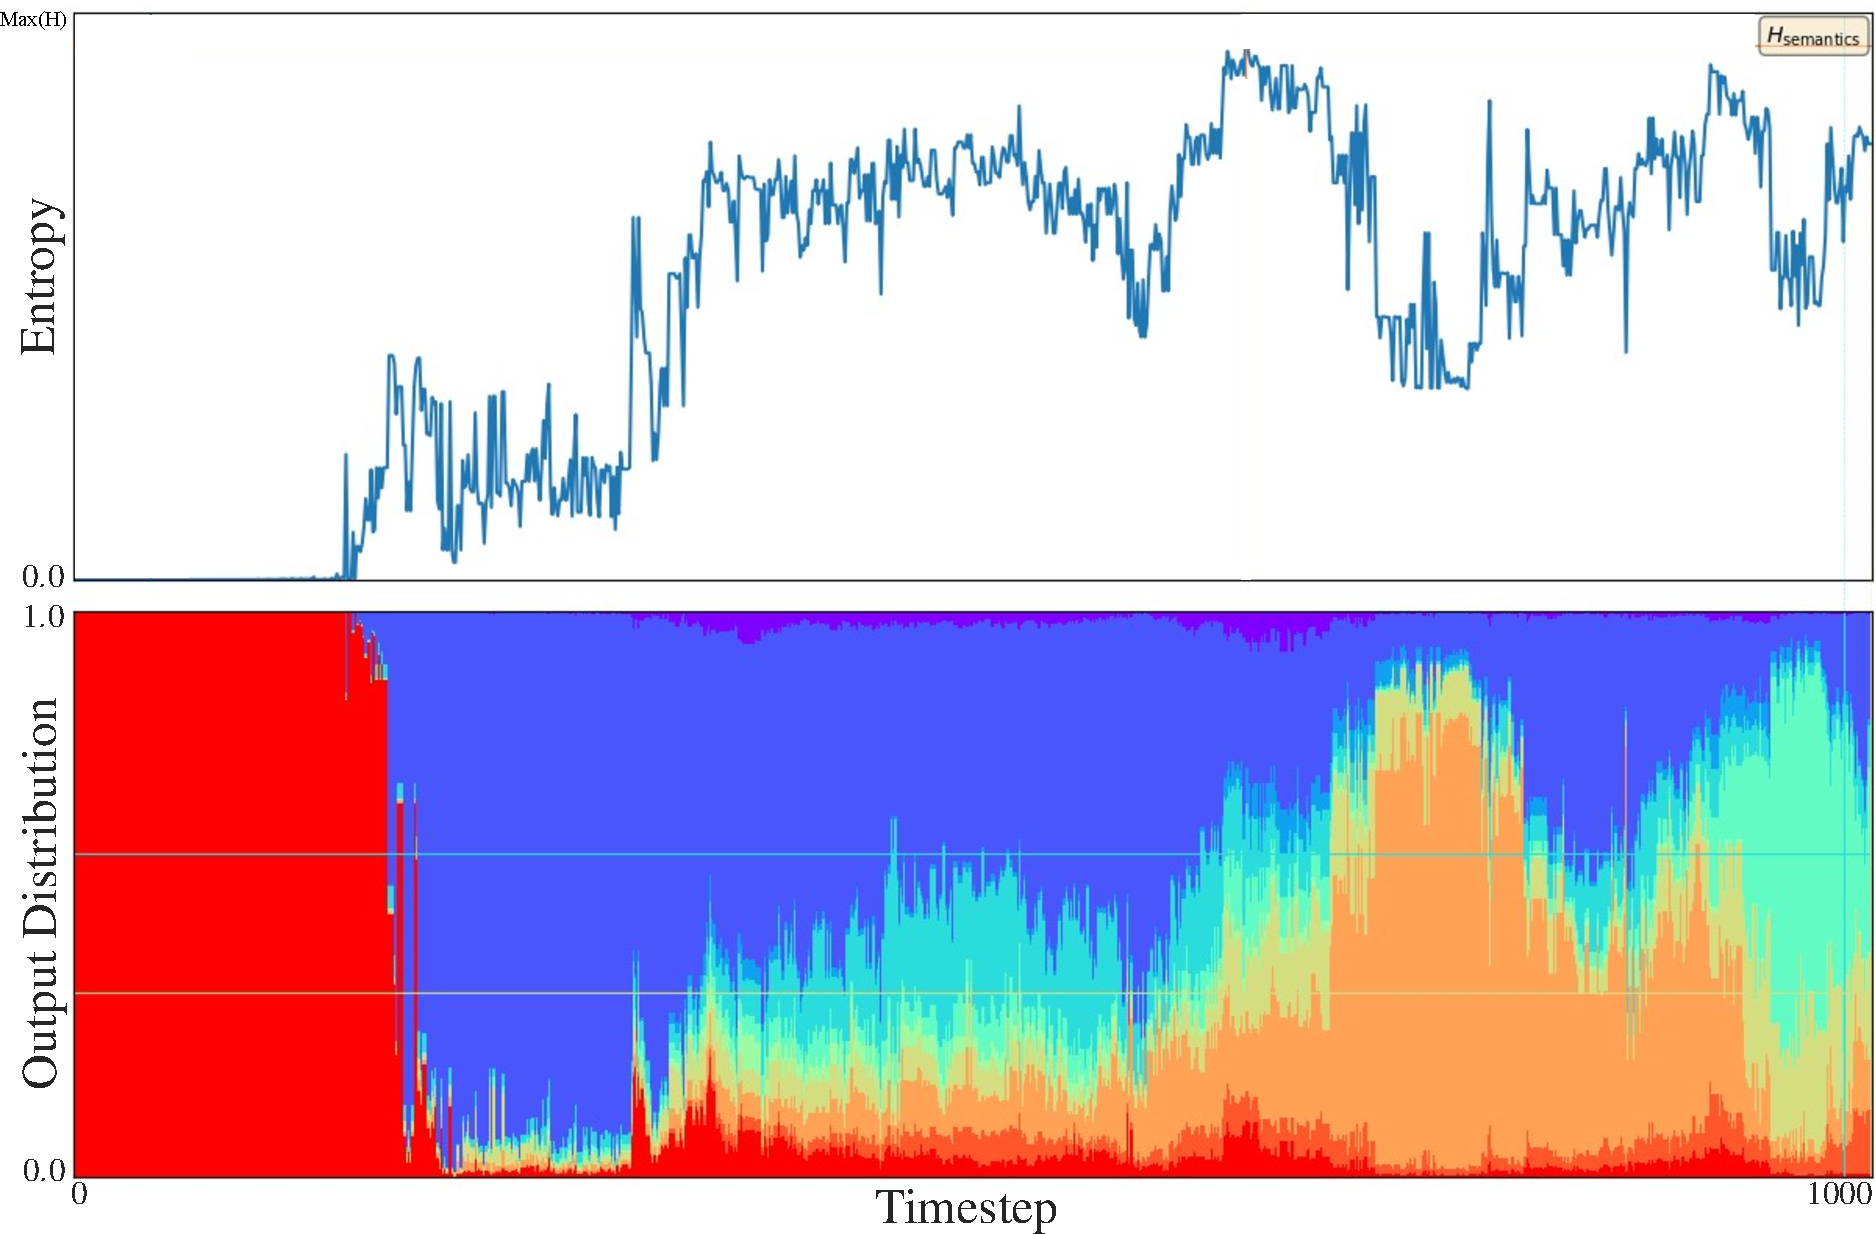
\includegraphics[width=0.8\textwidth]{images/Flatnet 15.pdf}
    \caption[A regular Flatnet MNIST classifier on random rollouts.]{A regular Flatnet MNIST classifier on random rollouts. Flatnet 15.}
    \vspace{12pt}
    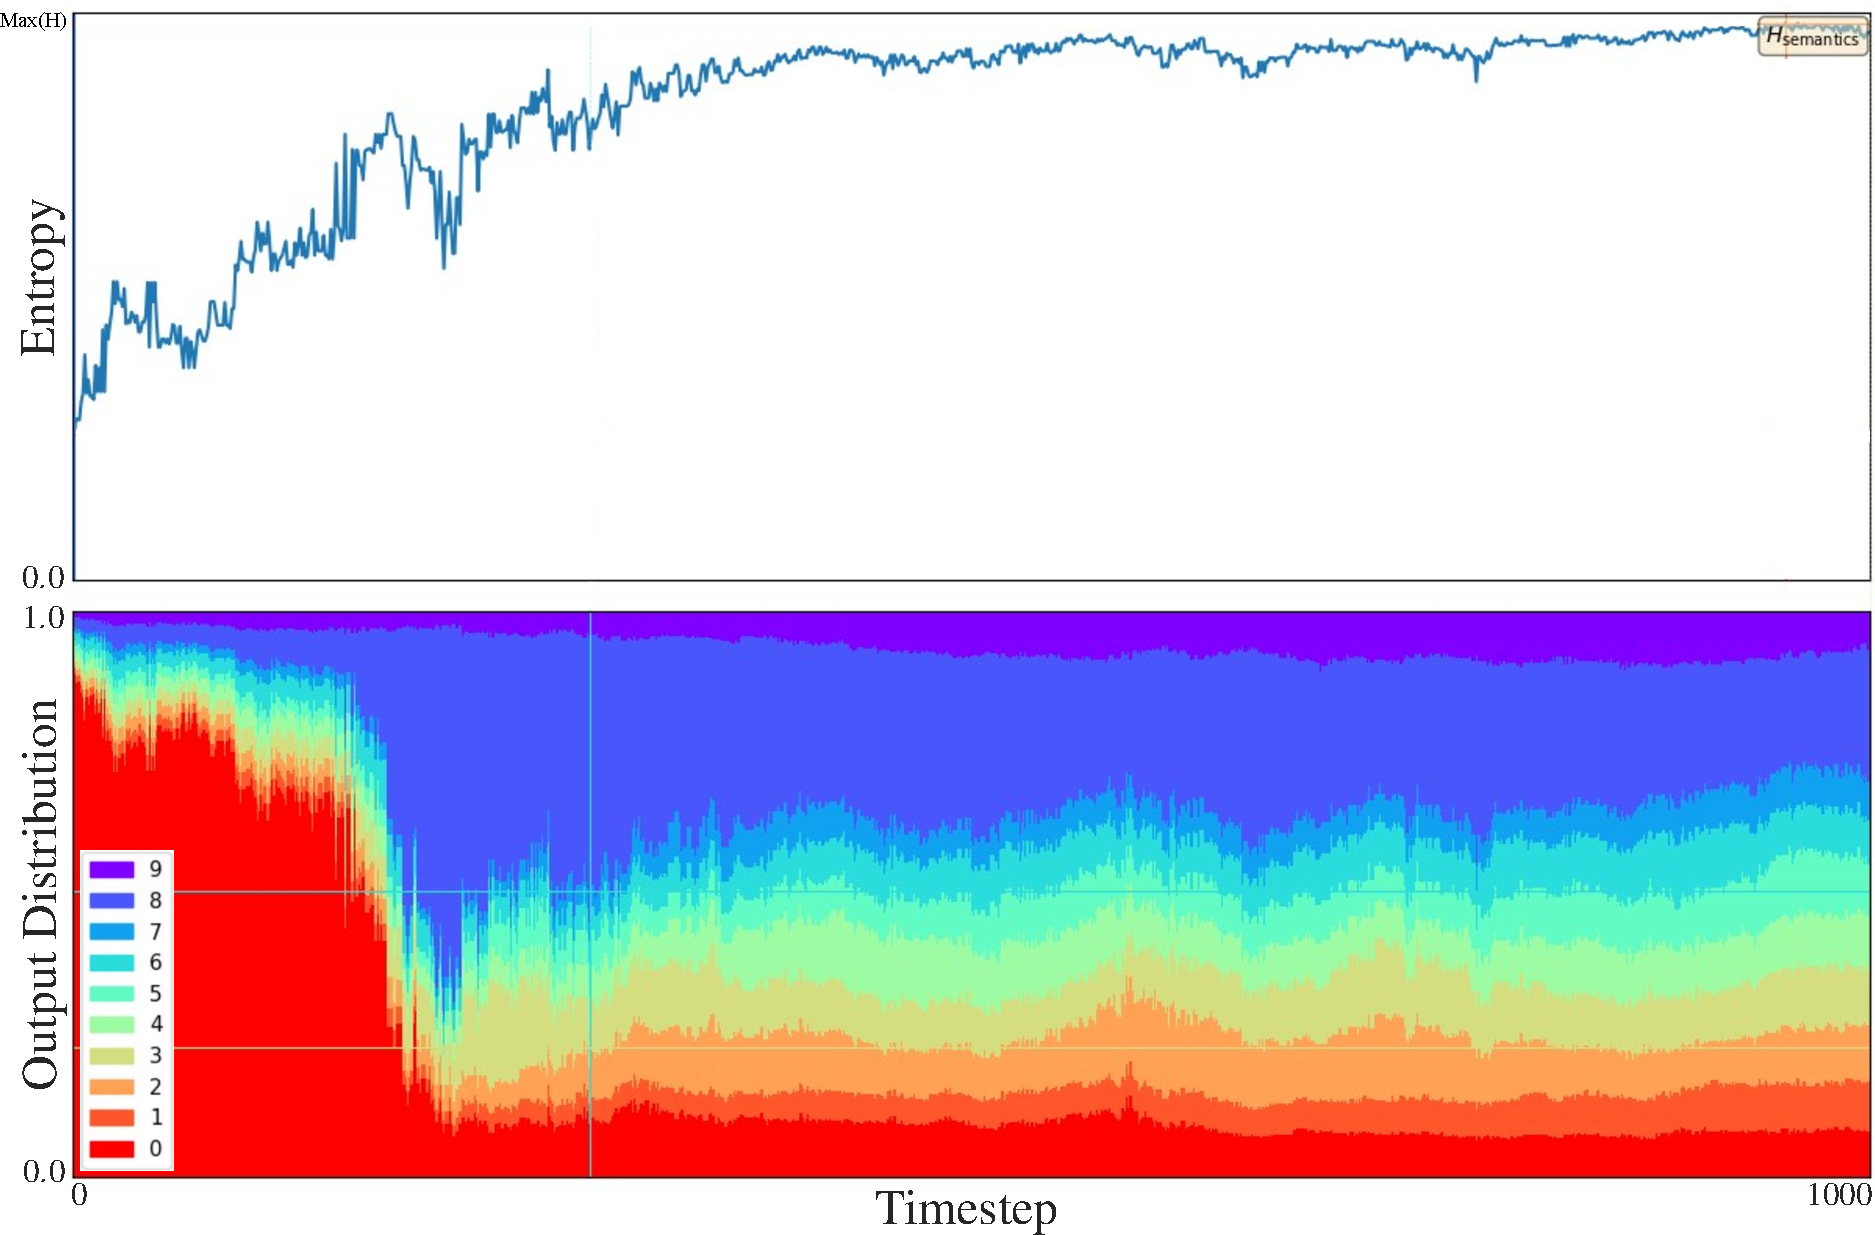
\includegraphics[width=0.8\textwidth]{images/Flatnet 3.pdf}
    \caption[An entropy regularized Flatnet MNIST classifier on random rollouts.]{An entropy regularized Flatnet MNIST classifier on random rollouts. Flatnet 3.}
    \label{fig:flatnet-comparison}
\end{figure}

Both, the entropy regularization and the addition of random samples, helped improve the reward trajectories of the models.
The regularized models have smoother entropy transitions, a stable distribution over time, and a flatter distribution (high entropy) for false positive (random) samples.


% \chapter{Descriptive List of Main Hyperparameters}
% \label{sec:hyperparameters}
% Here, we provide a list of the hyperparameters we mainly considered in our experiments.


\chapter{Improving Simulation Times}
\label{sec:efficiency}
Rendering the environment and using CLIP for planning was a very resource-intensive operation.
At every planning step, a total of \(\text{n\_trajectories} \times \text{horizon} \times \text{n\_icem\_inner\_iterations}\) evaluations needed to be computed.
This was further multiplied by the number of steps in the simulation.
This total ranged anywhere from \(~200,000\) to \(~2,000,000\) in our many experiments which corresponded to about \(2\) to \(20\) hours of simulation time if run in a single batch of inference on multiple GPUs.

Reducing simulation time was critical for us to be able to do any hyperparameter analysis.
We implemented several optimization techniques to improve this, which mainly involved efficient \emph{vectorization} of all computations, lazy evaluation, caching, parallelization, and cutting down on redundant operations.
In particular, two of these, for rendering and inference, are briefly introduced in the following sections.

\section{Reducing Rendering Time}
\label{sec:improving-render}
The rendering time was a major bottleneck for the simulations.
To improve this, we experimented with three popular open-source graphics Python libraries; \emph{Matplotlib} \citep{matplotlib}, \emph{Scikit-Image} \citep{skimage}, and \emph{OpenCV} \citep{opencv}, for both colored and grayscale renderings.
We used their functions in different formulations to further optimize their use.
The results of the best formulation for each of these libraries are summarized in \tabref{tab:render-time-color} and \tabref{tab:render-time-bw}.\\

\begin{table}[H]
    \centering
    \caption{Colored rendering-time comparison.}
    \begin{tabular}[t]{@{} c c c @{}}
        \hline
        \textbf{Library} & \textbf{Main Function/Class} & \textbf{Time (\(\mu s\))*}\\
        \hline
        Matplotlib & \texttt{PatchCollection} & 14400 ± 153\\
        Scikit-Image & \texttt{draw.polygon} & 978 ± 10.8\\
        OpenCV & \texttt{fillPoly} & 66.3 ± 0.85\\
        \hline
    \end{tabular}
    \label{tab:render-time-color}
\end{table}
\begin{table}[H]
    \centering
    \caption{Grayscale rendering-time comparison.}
    \begin{tabular}[t]{@{} c c c @{}}
        \hline
        \textbf{Library} & \textbf{Main Function/Class} & \textbf{Time (\(\mu s\))*}\\
        \hline
        Matplotlib & \texttt{PatchCollection} & 14200 ± 156\\
        Scikit-Image & \texttt{draw.polygon} & 978 ± 10.8\\
        OpenCV & \texttt{fillConvexPoly} & 52.2 ± 1.04\\
        \hline
    \end{tabular}
    \label{tab:render-time-bw}
\end{table}
* - Mean \(\pm\) standard deviation of \(7\) runs; \(1,000 - 10,000\) loops each.

These results refer to the Tangram environment, but the trend was the same with ShapeGridWorld.
The complete analysis is available on \url{https://github.com/pulkitgoyal56/master-thesis-notebooks/blob/main/archive/testbed_rendering.ignore.ipynb}.

\section{Reducing Inference Time}
\label{sec:improving-infer}
To minimize the inference times with CLIP, all inferences were done in one large batch.
This required significant memory, for which we parallelized them on multiple GPUs using Pytorch \texttt{DataParallel} \citep{pytorch}.

To reduce the inference time, we tweaked the image preprocessing functions of CLIP to be adaptive to the input to ensure that no redundant operations were performed.

Additionally, we picked the rendering configurations for the environments such that the resulting renders required minimal preprocessing in the form of resizing, cropping, type conversions, or copying, which was computationally expensive.
For example, all renderings concurred with the required input for the used CLIP model (eg. \(224 \times 224\) for the \texttt{ViT-L/14} variant) used for inference to avoid any resizing.
This also helped to improve the simulation times significantly.\\

\begin{figure}[H]
    \centering
    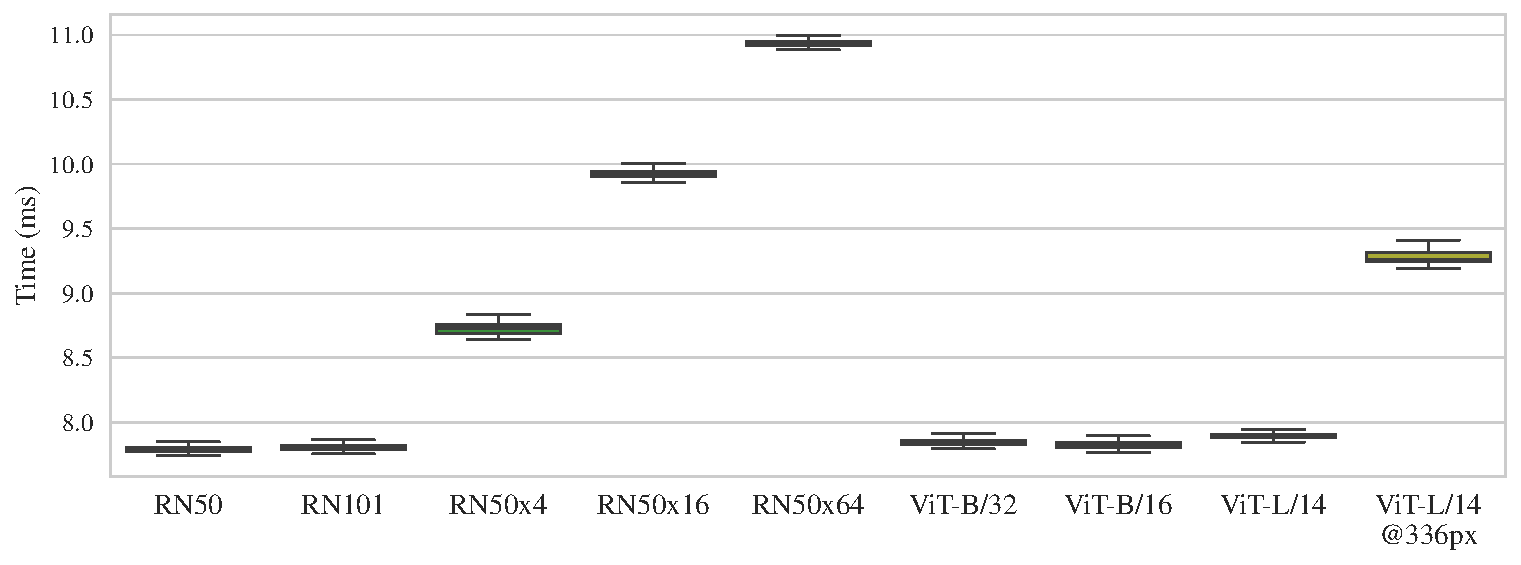
\includegraphics[width=\textwidth]{images/full_transform.pdf}
    \vspace{-12pt}
    \caption{Preprocessing times before optimizations.}
    \vspace{12pt}
    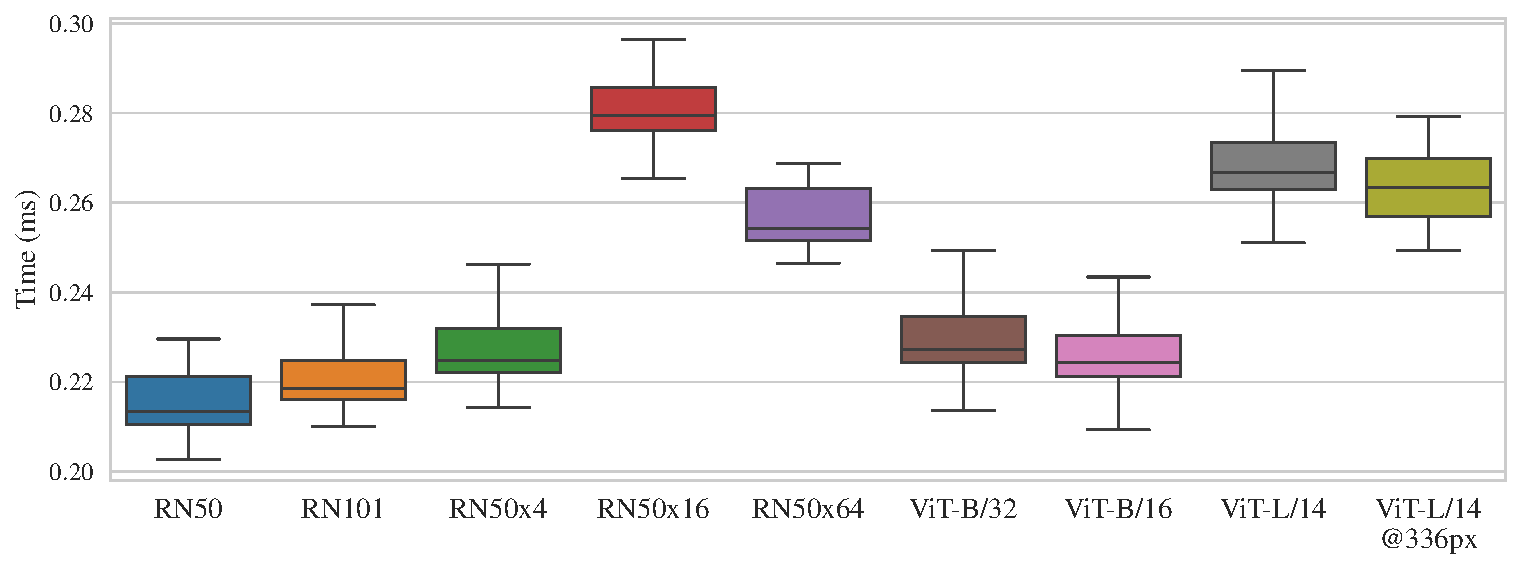
\includegraphics[width=\textwidth]{images/fast_transform.pdf}
    \vspace{-12pt}
    \caption{Preprocessing times after optimizations.}
    \label{fig:preprocessing-time-improvement}
\end{figure}

These modifications are available on \url{https://github.com/pulkitgoyal56/CLIP/tree/preprocess-tweaks}.



\chapter{Additional Simulations on ShapeGridWorld}
\label{sec:sgw-semantics-additional}

\section{Effect of Semantic Categories Set}
\label{sec:sgw-categories}
The effect of the choice of categories on the semantics entropy reward in ShapeGridWorld was also significant.
\figref{fig:categories-sgw} and \figref{fig:categories-sgw-norair} show the effect of different sets of categories on the reward landscape and some samples of their creations, with and without RaIR respectively.

We observe that categories involving numbers (``numbers and letters'' and ``numbers'') start with a flatter distribution compared to object categories (few or many).

% categories_boxplot_sgw_rair.pdf
% categories_comparison_sgw_rair.pdf
% categories_samples_sgw_rair.pdf
\begin{figure}[h]
    \centering
    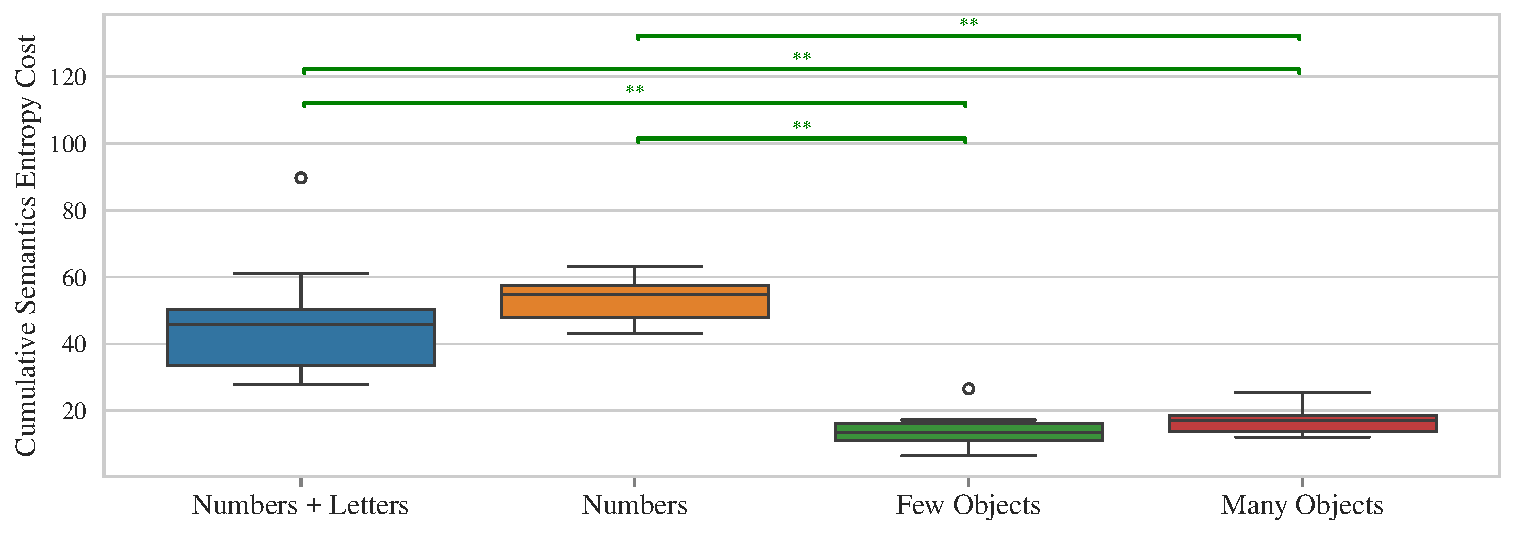
\includegraphics[width=\textwidth]{images/categories_boxplot_sgw_rair_cropped.pdf}
    % \label{fig:categories-boxplot-sgw}
    \vspace{12pt}
    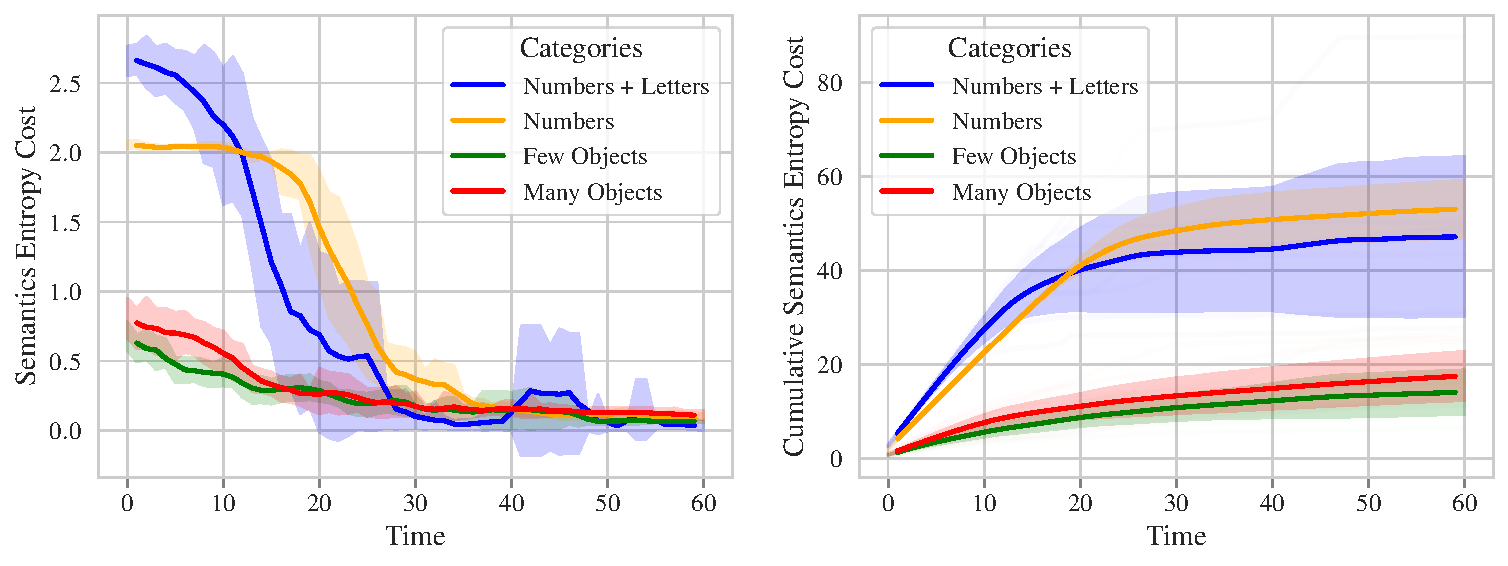
\includegraphics[width=\textwidth]{images/categories_comparison_sgw_rair.pdf}
    % \caption{Effect of categories on semantics entropy reward in ShapeGridWorld. 10 seeds were used.}
    \vspace{12pt}
    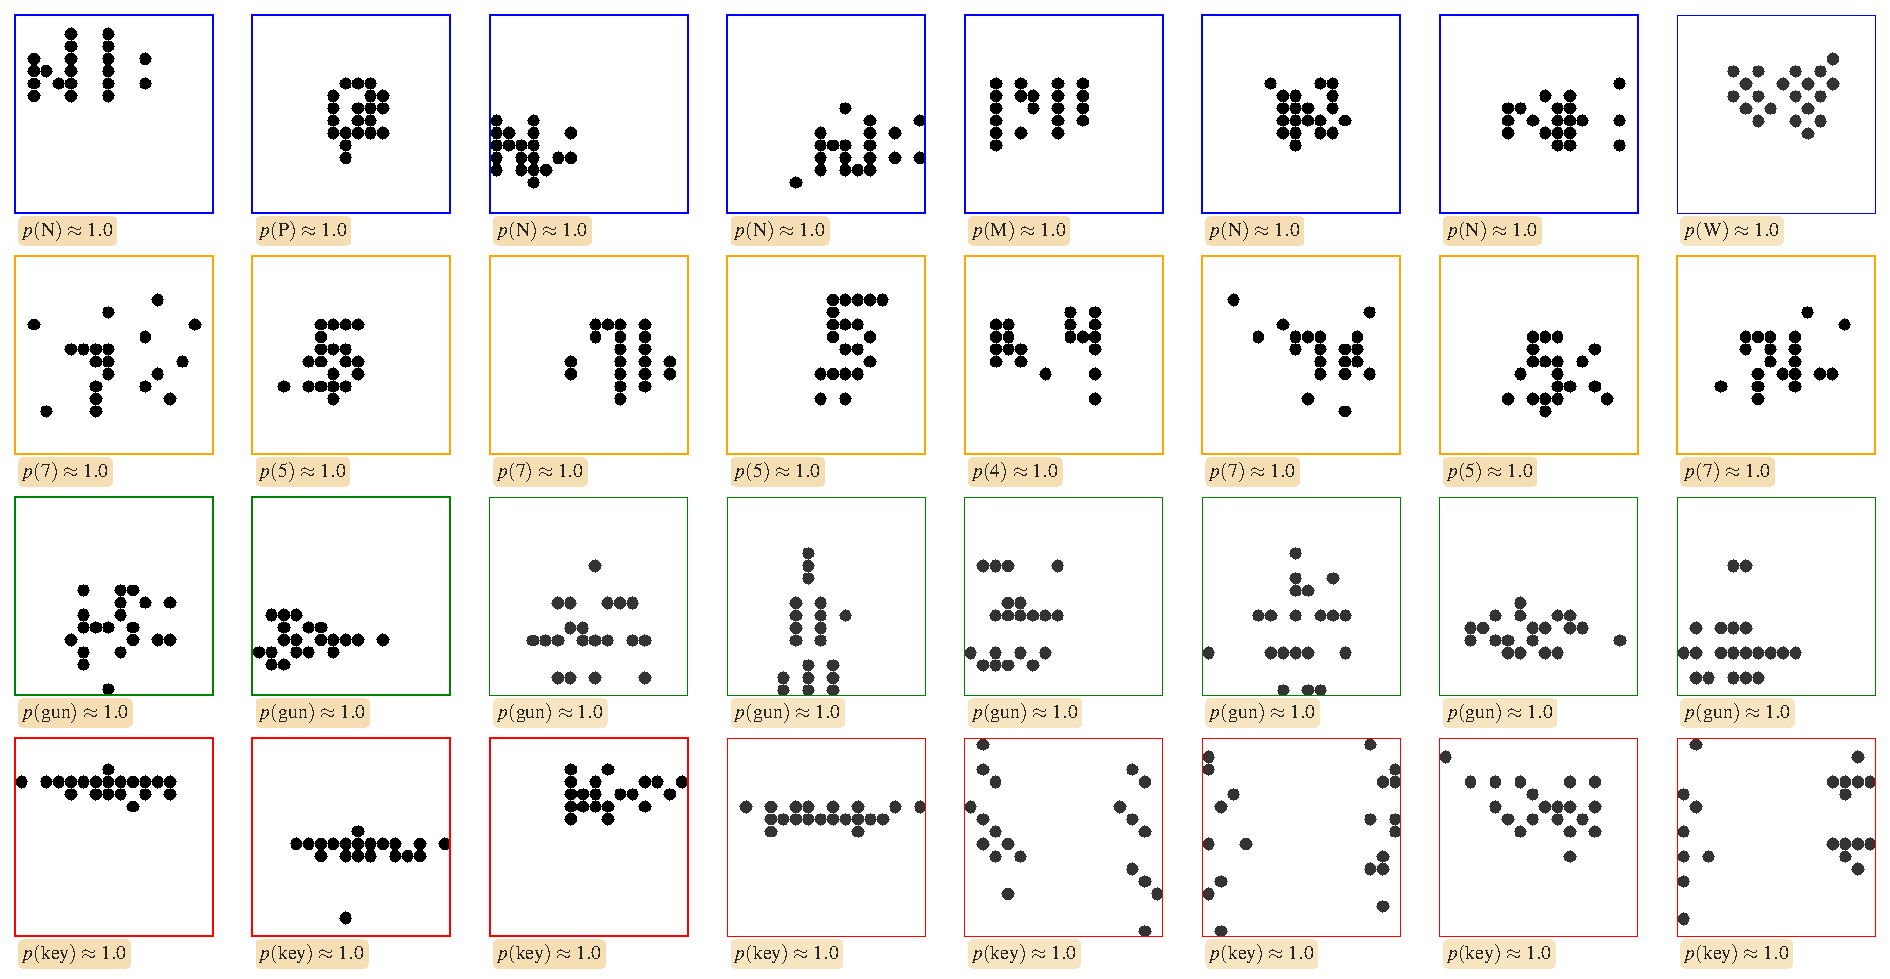
\includegraphics[width=\textwidth]{images/categories_samples_sgw_rair.pdf}
    % \caption{Samples of creations with different categories in ShapeGridWorld.}
    % \label{fig:categories-samples-sgw}
    \caption[Effect of categories on semantics entropy reward in ShapeGridWorld.]{Effect of categories on semantics entropy reward in ShapeGridWorld. 10 seeds were used.}
    \label{fig:categories-sgw}
\end{figure}

% categories_boxplot_sgw_norair.pdf
% categories_comparison_sgw_norair.pdf
% categories_samples_sgw_norair.pdf
\begin{figure}[h]
    \centering
    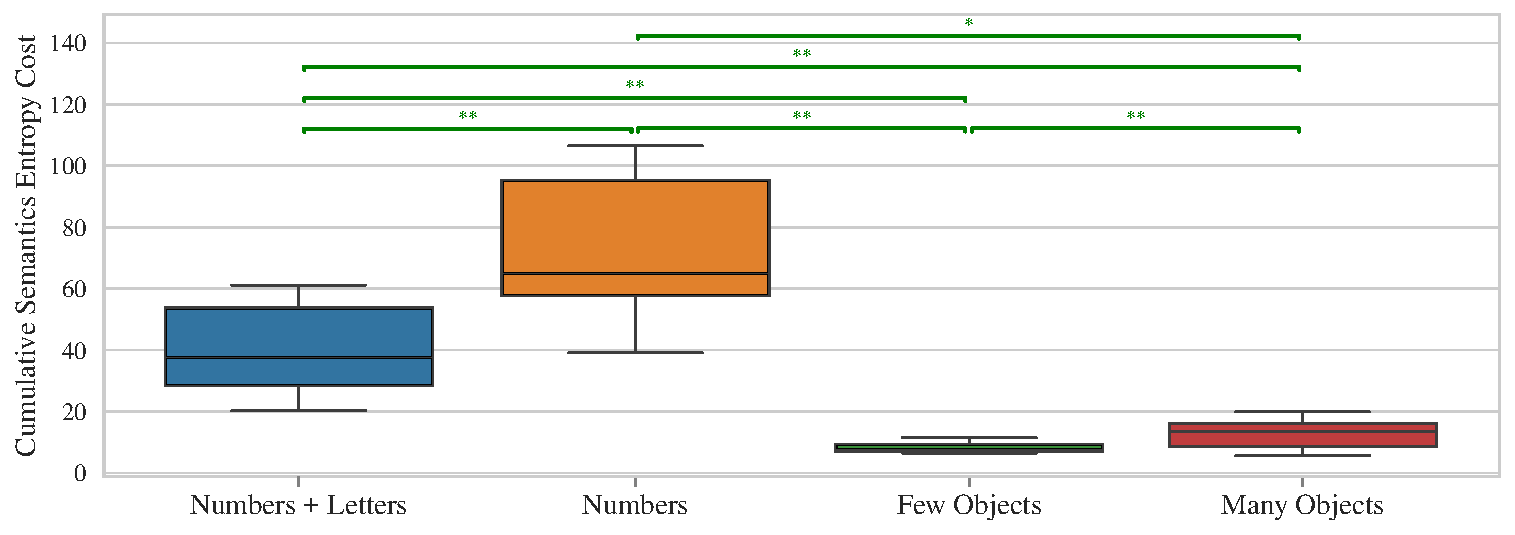
\includegraphics[width=\textwidth]{images/categories_boxplot_sgw_norair_cropped.pdf}
    % \label{fig:categories-boxplot-sgw-norair}
    \vspace{12pt}
    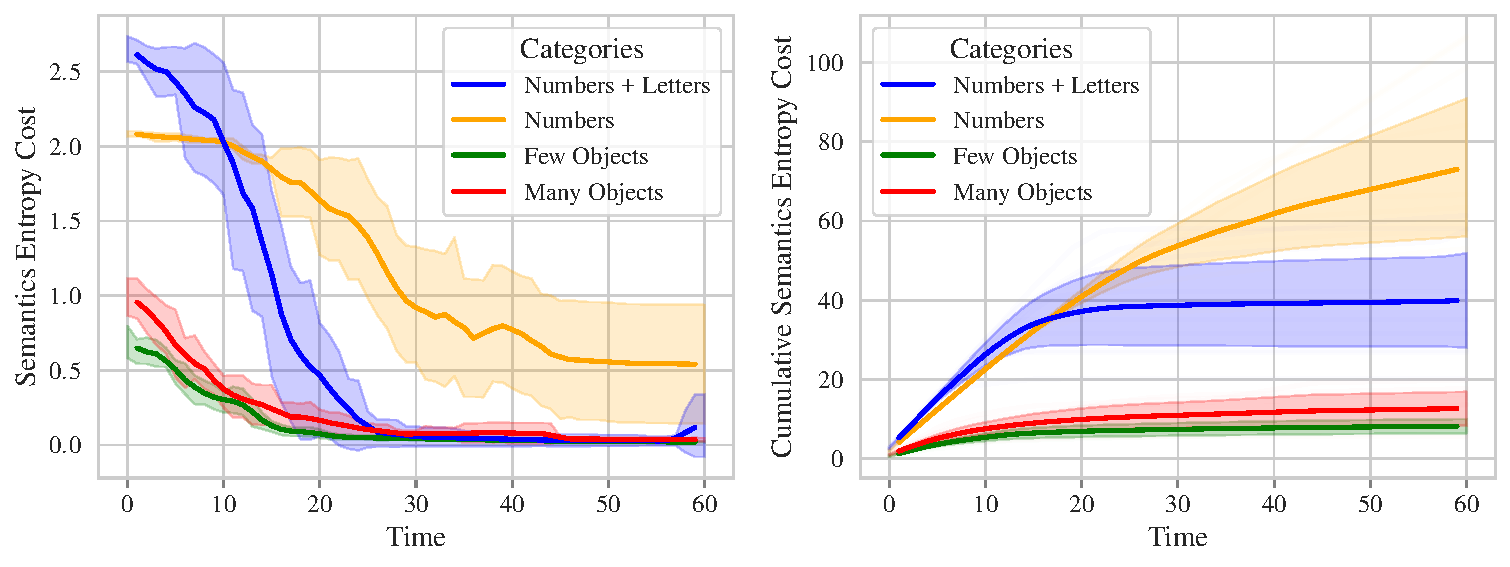
\includegraphics[width=\textwidth]{images/categories_comparison_sgw_norair_cropped.pdf}
    % \caption{Effect of categories on semantics entropy reward in ShapeGridWorld without RaIR. 10 seeds were used.}
    \vspace{12pt}
    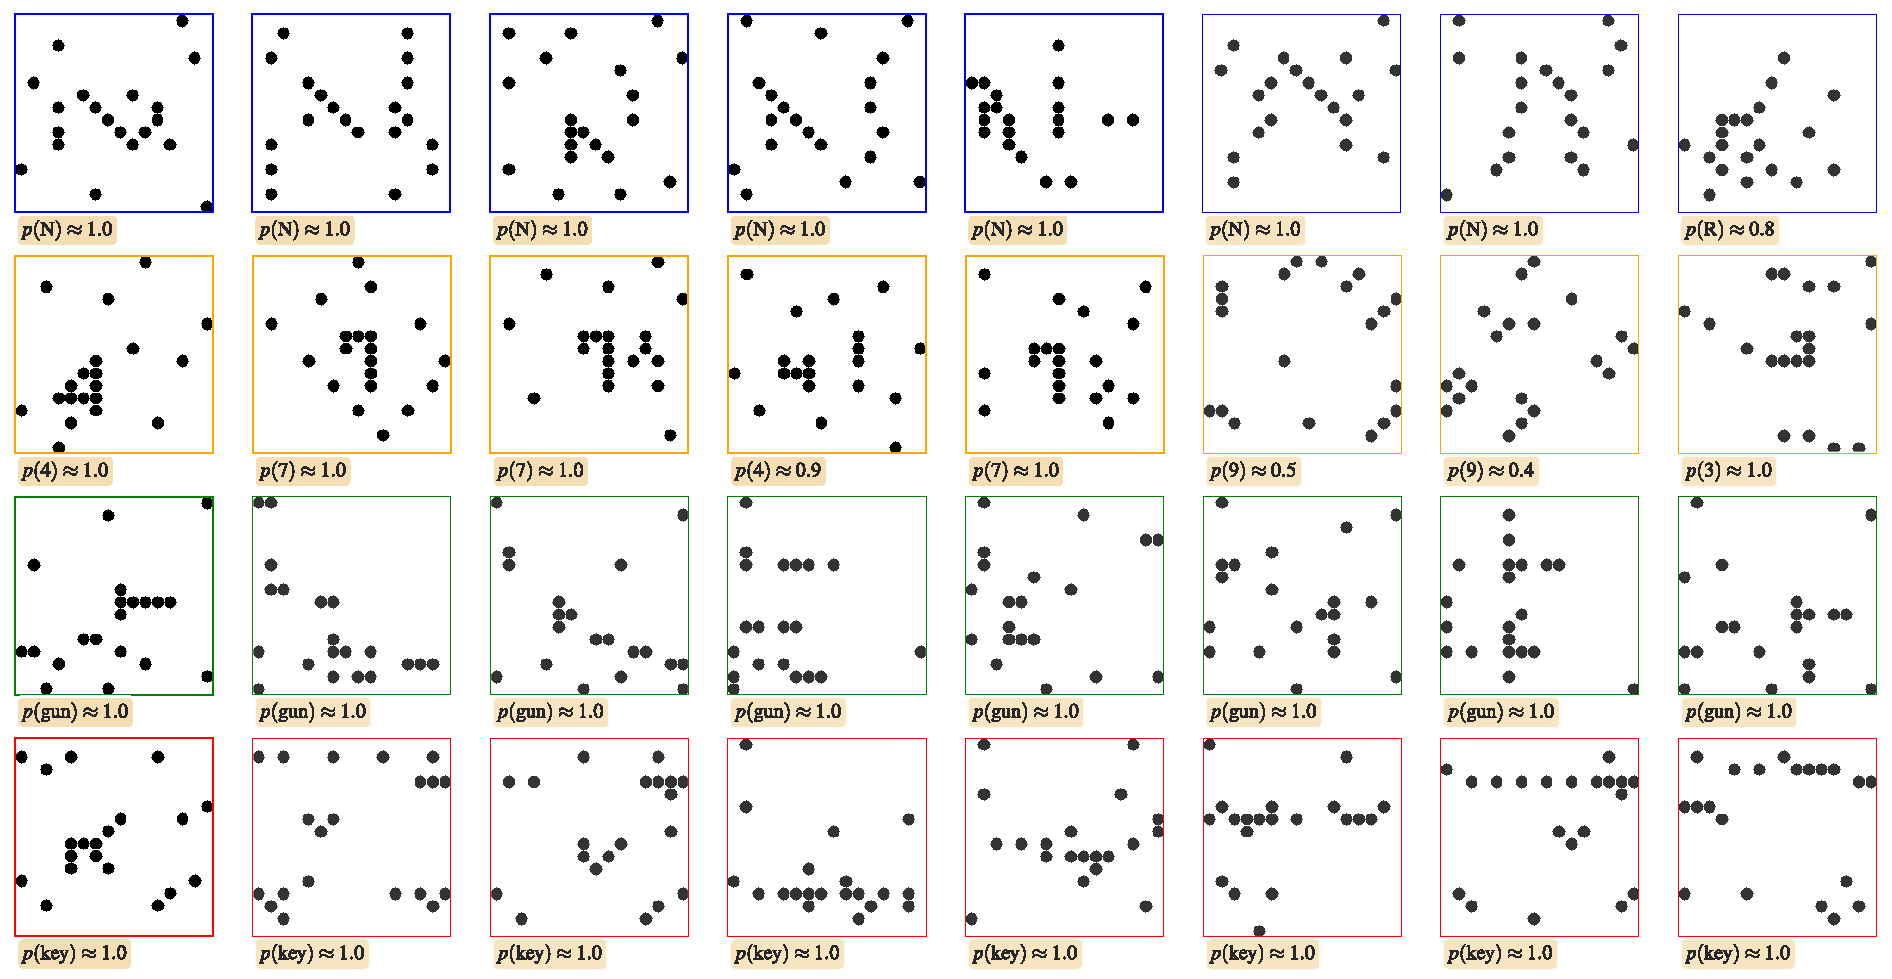
\includegraphics[width=\textwidth]{images/categories_samples_sgw_norair_cropped.pdf}
    % \caption{Samples of creations with different categories in ShapeGridWorld without RaIR.}
    % \label{fig:categories-samples-sgw-norair}
    \caption[Effect of categories on semantics entropy reward in ShapeGridWorld without RaIR.]{Effect of categories on semantics entropy reward in ShapeGridWorld without RaIR. 10 seeds were used.}
    \label{fig:categories-sgw-norair}
\end{figure}

\section{Effect of Grayscale Pixels}
\label{sec:sgw-grayscale}
% mode_comparison_sgw.pdf
% mode_samples_sgw.pdf
Observing the effect of the grayscale values on the effect of RaIR in ShapeGridWorld, we also ran simulations with different categories of colors in the pixels.

It seems that the presence of grayscale pixels has a regularizing effect on the reward landscape and consequently there is less noise in CLIP.
This is evident from the reduced confidence in the imperfect final creations in \figref{fig:mode-sgw}.

\begin{figure}[h]
    \centering
    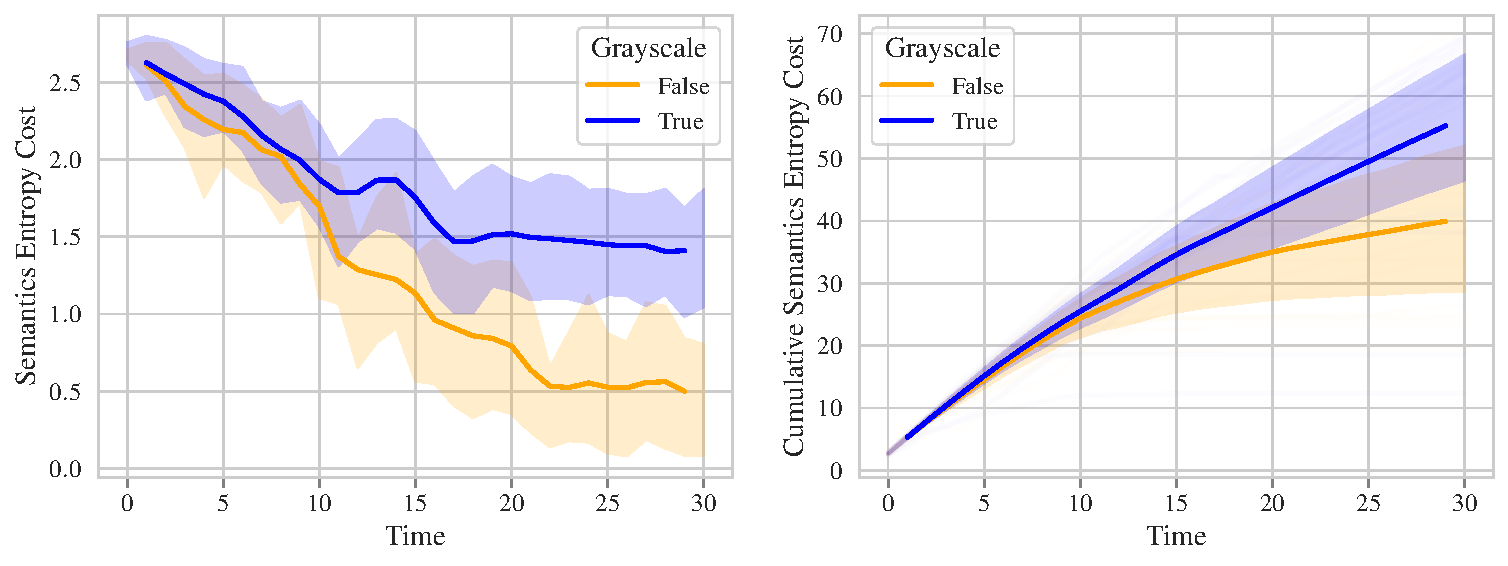
\includegraphics[width=\textwidth]{images/mode_comparison_sgw.pdf}
    \vspace{12pt}
    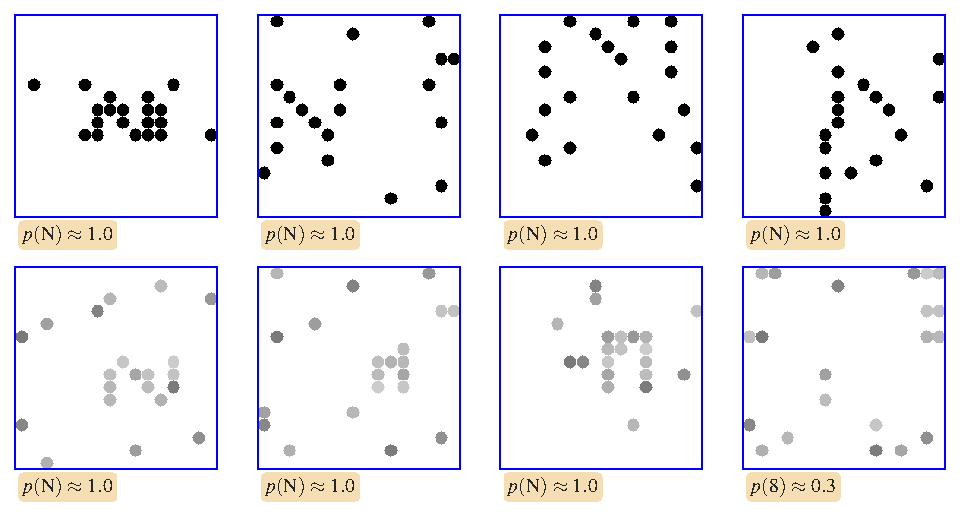
\includegraphics[width=0.66\textwidth]{images/mode_samples_sgw.pdf}
    % \caption{Samples of creations with and without grayscale pixels in ShapeGridWorld.}
    % \label{fig:mode-samples-sgw}
    \caption{Effect of the presence of grayscale pixels on semantics entropy reward in ShapeGridWorld.}
    \label{fig:mode-sgw}
\end{figure}

\section{Effect of Number of Pixels}
\label{sec:sgw-pixels}
% Threshold Ratio
% n_objects_comparison_sgw.pdf
% n_objects_samples_sgw.pdf

As we noted earlier, the presence of a high number of controllable pixels in the ShapeGridWorld exacerbates the problem of noise in CLIP and is also a more difficult control problem, hence we also experimented with different numbers of pixels in the environment.

Having too few pixels also results in a rather noisy landscape with a lot of false positives, as seen in \figref{fig:n-objects-sgw}.
This seems to suggest that moderate numbers of pixels are optimal for the environment.

\begin{figure}[h]
    \centering
    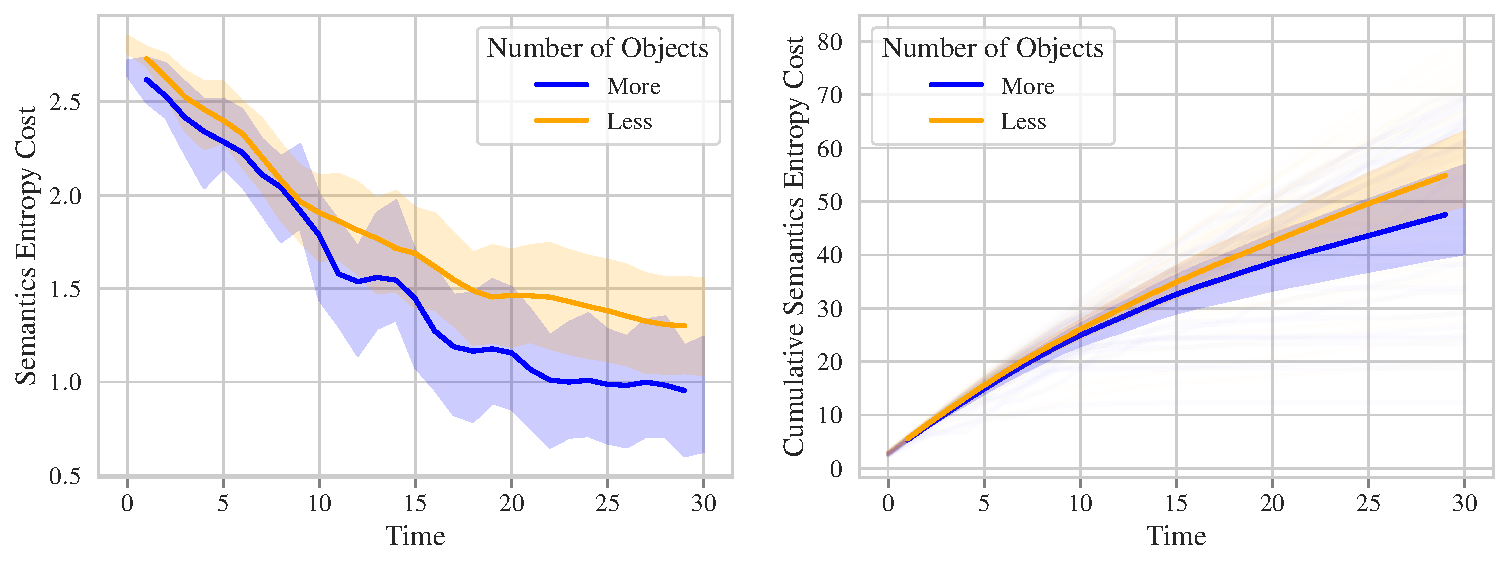
\includegraphics[width=\textwidth]{images/n_objects_comparison_sgw.pdf}
    \vspace{12pt}
    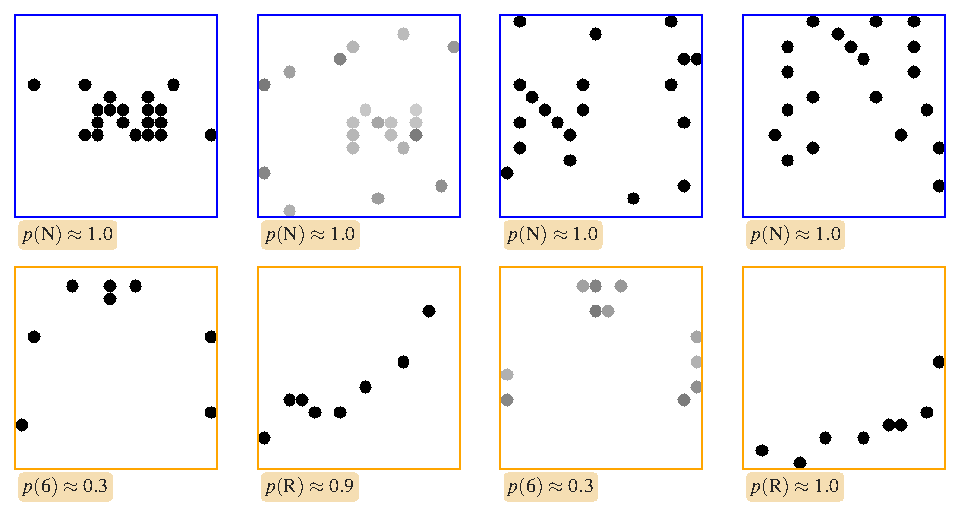
\includegraphics[width=0.66\textwidth]{images/n_objects_samples_sgw.pdf}
    % \caption{Samples of creations with different numbers of objects in ShapeGridWorld.}
    % \label{fig:n-objects-samples-sgw}
    \caption{Effect of the number of objects on semantics entropy reward in ShapeGridWorld.}
    \label{fig:n-objects-sgw}
\end{figure}

% nobj_mode_rair_sgw_boxplot.pdf
The effects of the number of objects, grayscale pixels, and RaIR are summarised in \figref{fig:nobj-mode-sgw}
\begin{figure}[h]
    \centering
    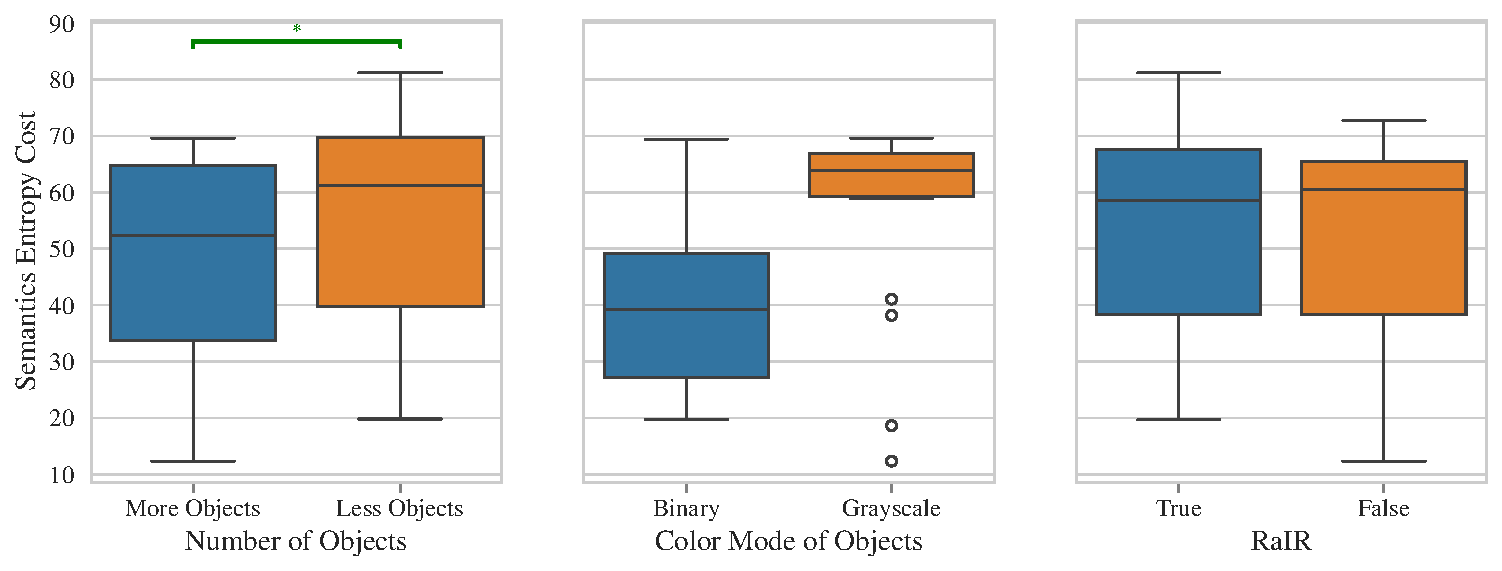
\includegraphics[width=\textwidth]{images/nobj_mode_rair_sgw_boxplot.pdf}
    \caption{Effect of the number of objects, grayscale pixels, and RaIR on semantics entropy reward in ShapeGridWorld.}
    \label{fig:nobj-mode-sgw}
\end{figure}

\newpage
\section{Effect of Object Persistency}
\label{sec:sgw-persistency}
% Object Persistency
% object_persistency_comparison_sgw.pdf
% object_persistency_samples_sgw.pdf

We also experimented with the ``object persistency'' of objects in the environment, which defines how many action steps an object is moved before the controller switches its focus on the next object in the predetermined order.
This also included the case of moving all the objects together.
This is related to the step size of the environment which defines how many steps in x/y-directions an object can be moved in one action.

Since the action space with moving all the objects at the same time can be very large (proportional to the number of objects), the controller needs more computational budget to realize the optimal policy, in the form of a higher planning horizon, more sampled trajectories, or more iterations to converge.
We noticed that we obtained the best results when the objects were moved one at a time, only for one timestep, i.e. an object persistency of \(1\), with a step size around a quarter of the grid size.
This is evident from the faster convergence in \figref{fig:object-persistency-sgw}.

\begin{figure}[h]
    \centering
    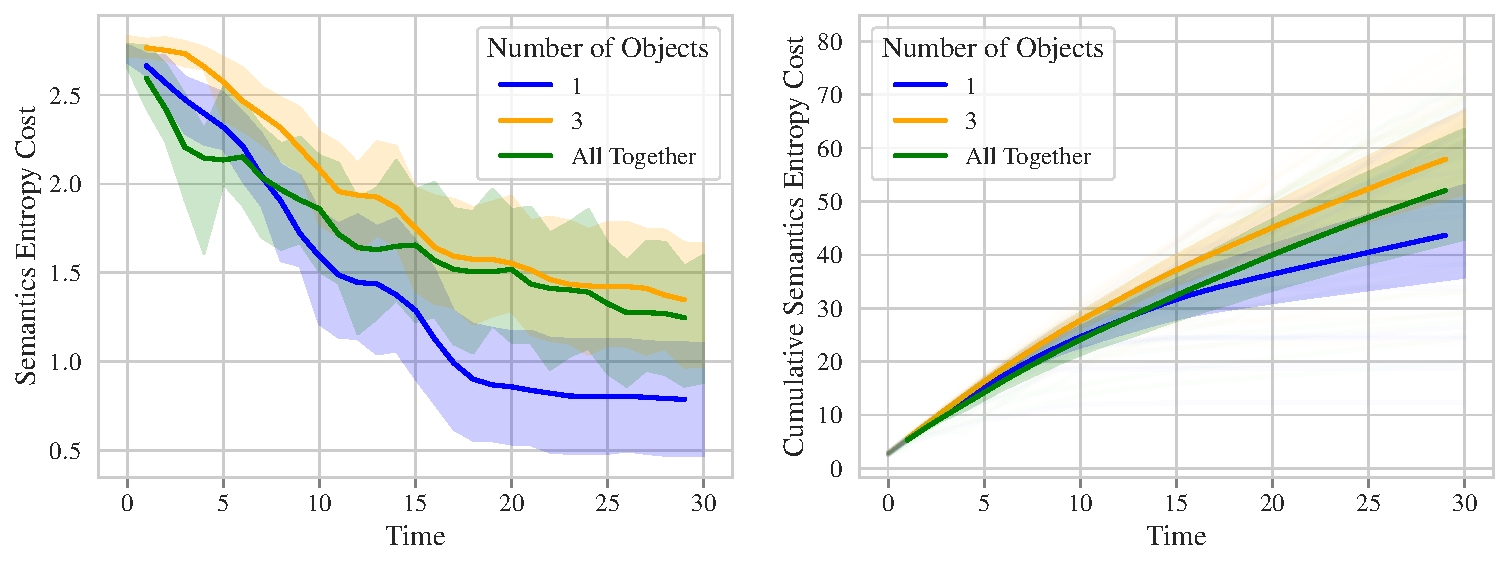
\includegraphics[width=\textwidth]{images/object_persistency_comparison_sgw.pdf}
    \vspace{12pt}
    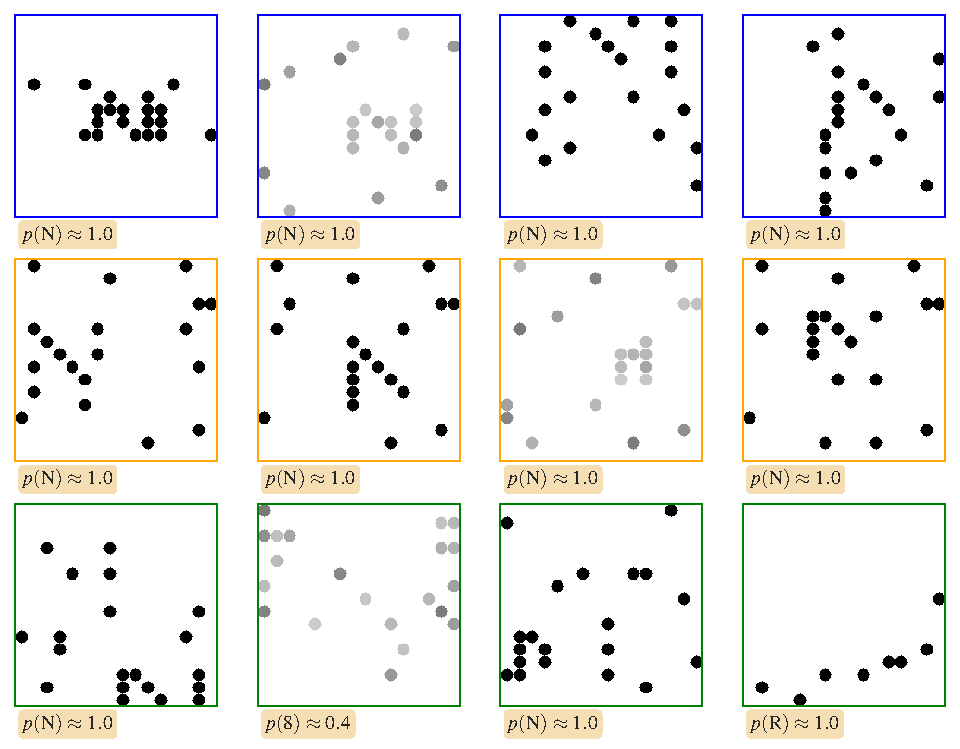
\includegraphics[width=0.66\textwidth]{images/object_persistency_samples_sgw.pdf}
    % \caption{Samples of creations with different object persistency in ShapeGridWorld.}
    % \label{fig:object-persistency-samples-sgw}
    \caption{Effect of object persistency on semantics entropy reward in ShapeGridWorld.}
    \label{fig:object-persistency-sgw}
\end{figure}


\chapter{Additional Graphs}
\label{sec:additional-graphs}

% Class preference in CLIP
\begin{figure}[h]
    \centering
    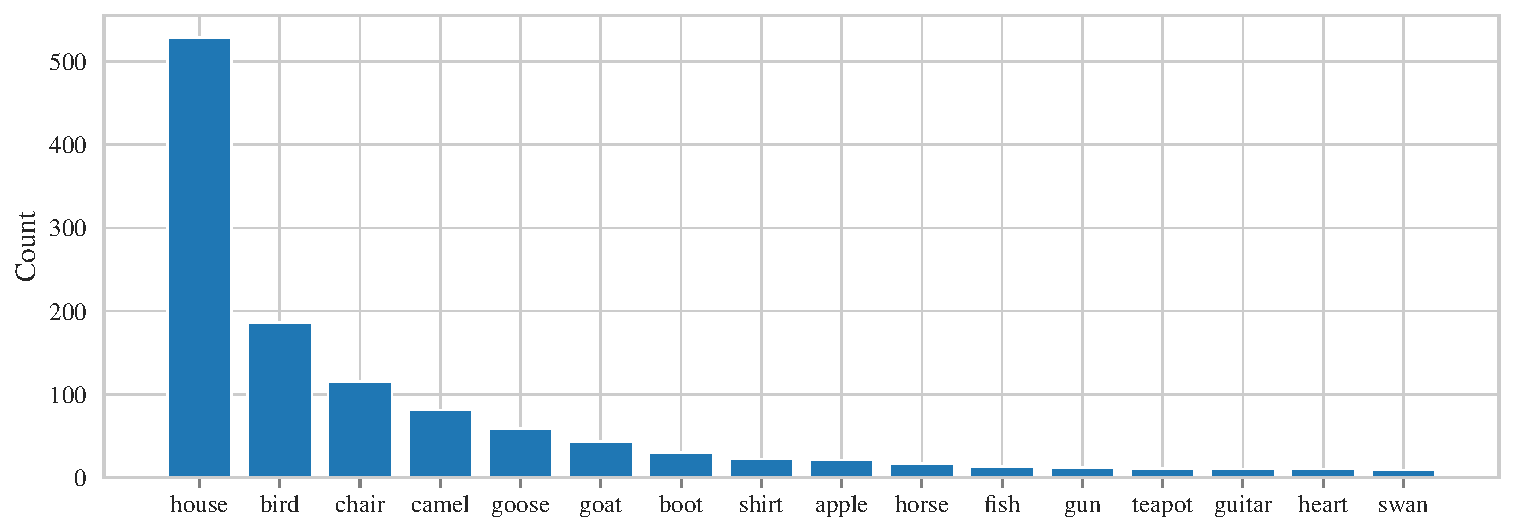
\includegraphics[width=\textwidth]{images/creations_distribution.pdf}
    \vspace{-12pt}
    \caption[Histogram of creations in our simulations on Tangram showing CLIP's class preference.]{Histogram of creations in our simulations on Tangram showing CLIP's class preference. The choice of classes varied in these simulations; when ``house'' or ``bird'' were present, they were chosen almost all the time. The other creations were obtained only when they were removed. Classes not mentioned in the graph include ``boat'', ``teapot'', ``gun'', ``car'', ``airplane'', ``guitar'', and ``flower''}
    \label{fig:class-preference-tangram}
    \vspace{12pt}
    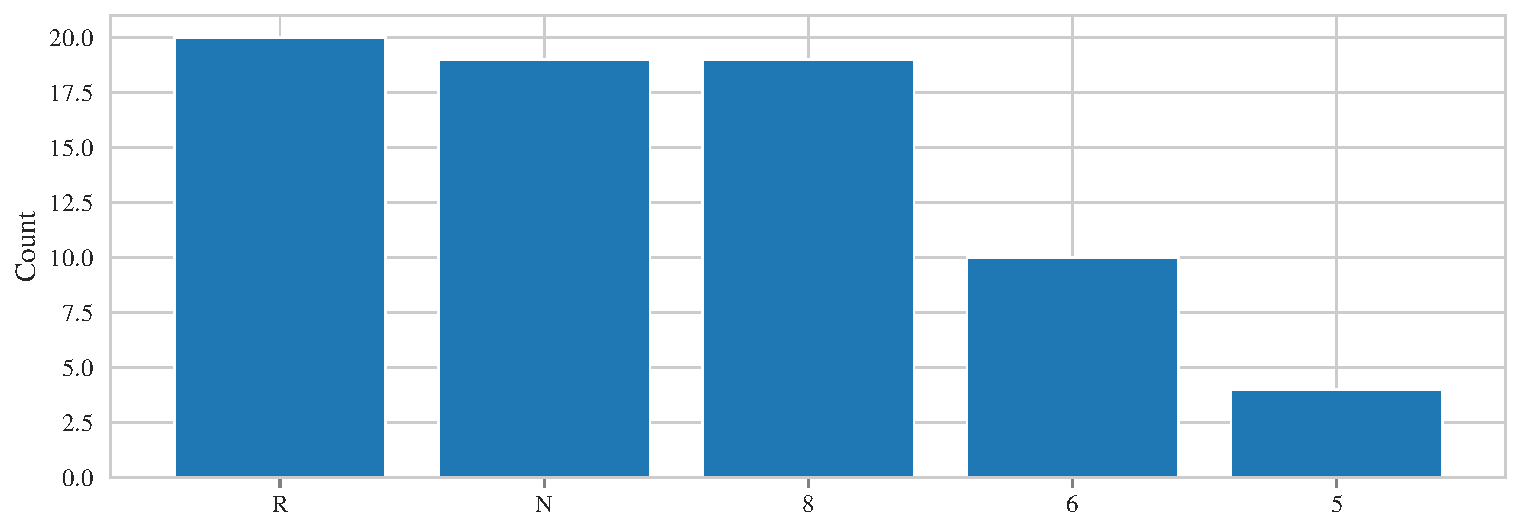
\includegraphics[width=\textwidth]{images/creations_distribution_sgw.pdf}
    \vspace{-12pt}
    \caption[Histogram of creations in our simulations on ShapeGridWorld showing CLIP's class preference.]{Histogram of creations in our simulations on ShapeGridWorld showing CLIP's class preference. The \(36\) classes are all letters and numbers.}
    \label{fig:class-preference-sgw}
\end{figure}

% % alpha_beta-semantics_std_rair.pdf
% \begin{figure}[h]
%     \centering
%     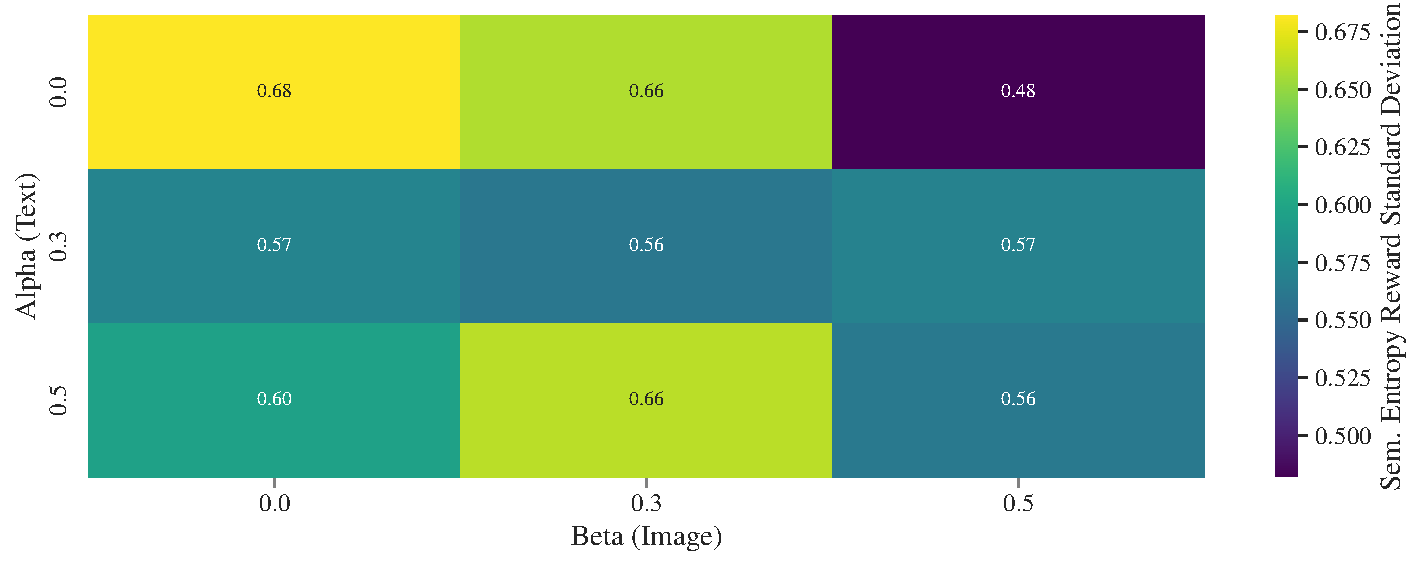
\includegraphics[width=0.96\textwidth]{images/alpha_beta-semantics_std_rair.pdf}
%     \caption{Standard deviation of regularization strength performance on the semantics reward.}
%     \label{fig:alpha_beta-semantics_std_rair}
% \end{figure}

% all inversions of an image
\begin{figure}[h]
    \centering
    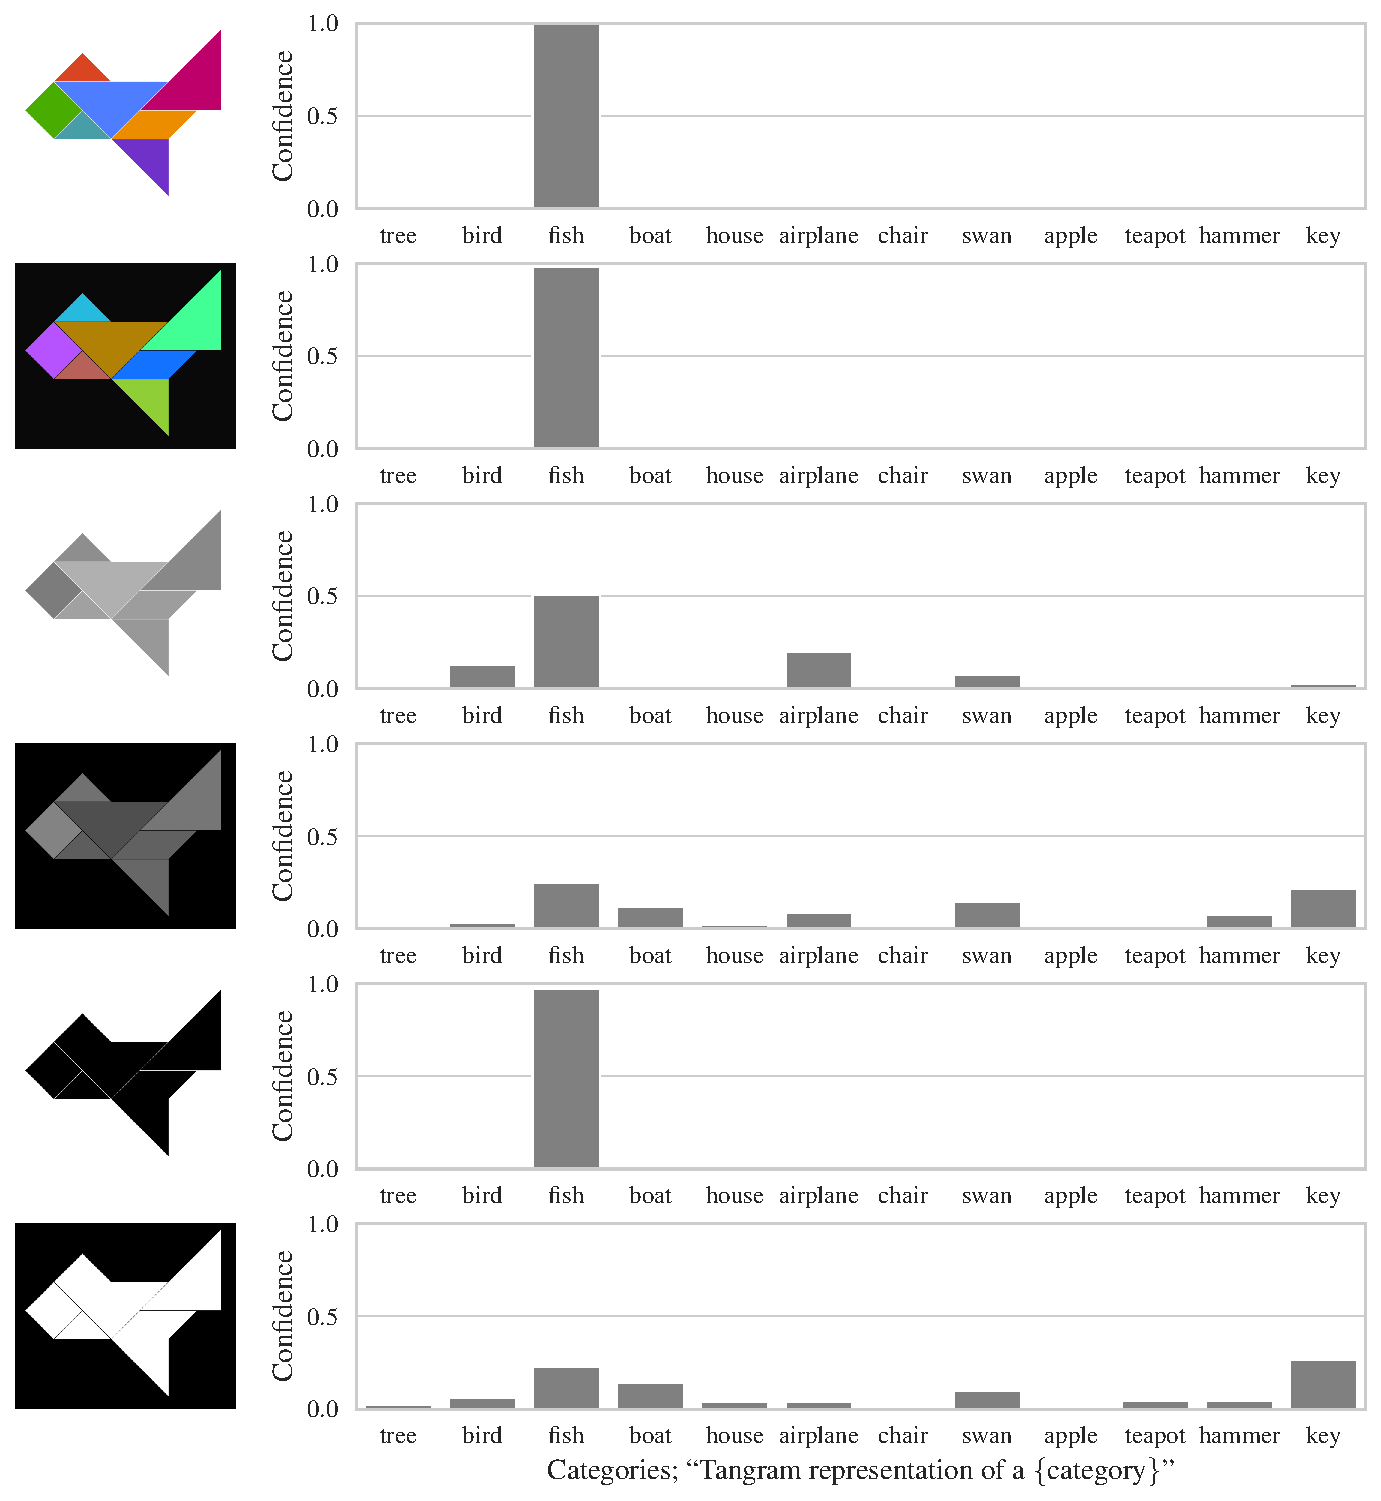
\includegraphics[width=0.95\textwidth]{images/tangram_fish_10.pdf}
    \caption{CLIP on different inversions of the same Tangram creation. \(T = 0.1\).}
    \label{fig:clip-tangram-inversions}
\end{figure}


\chapter{Curated Gallery}
\label{sec:gallery}

% curation_bird.pdf
\begin{figure}[H]
    \centering
    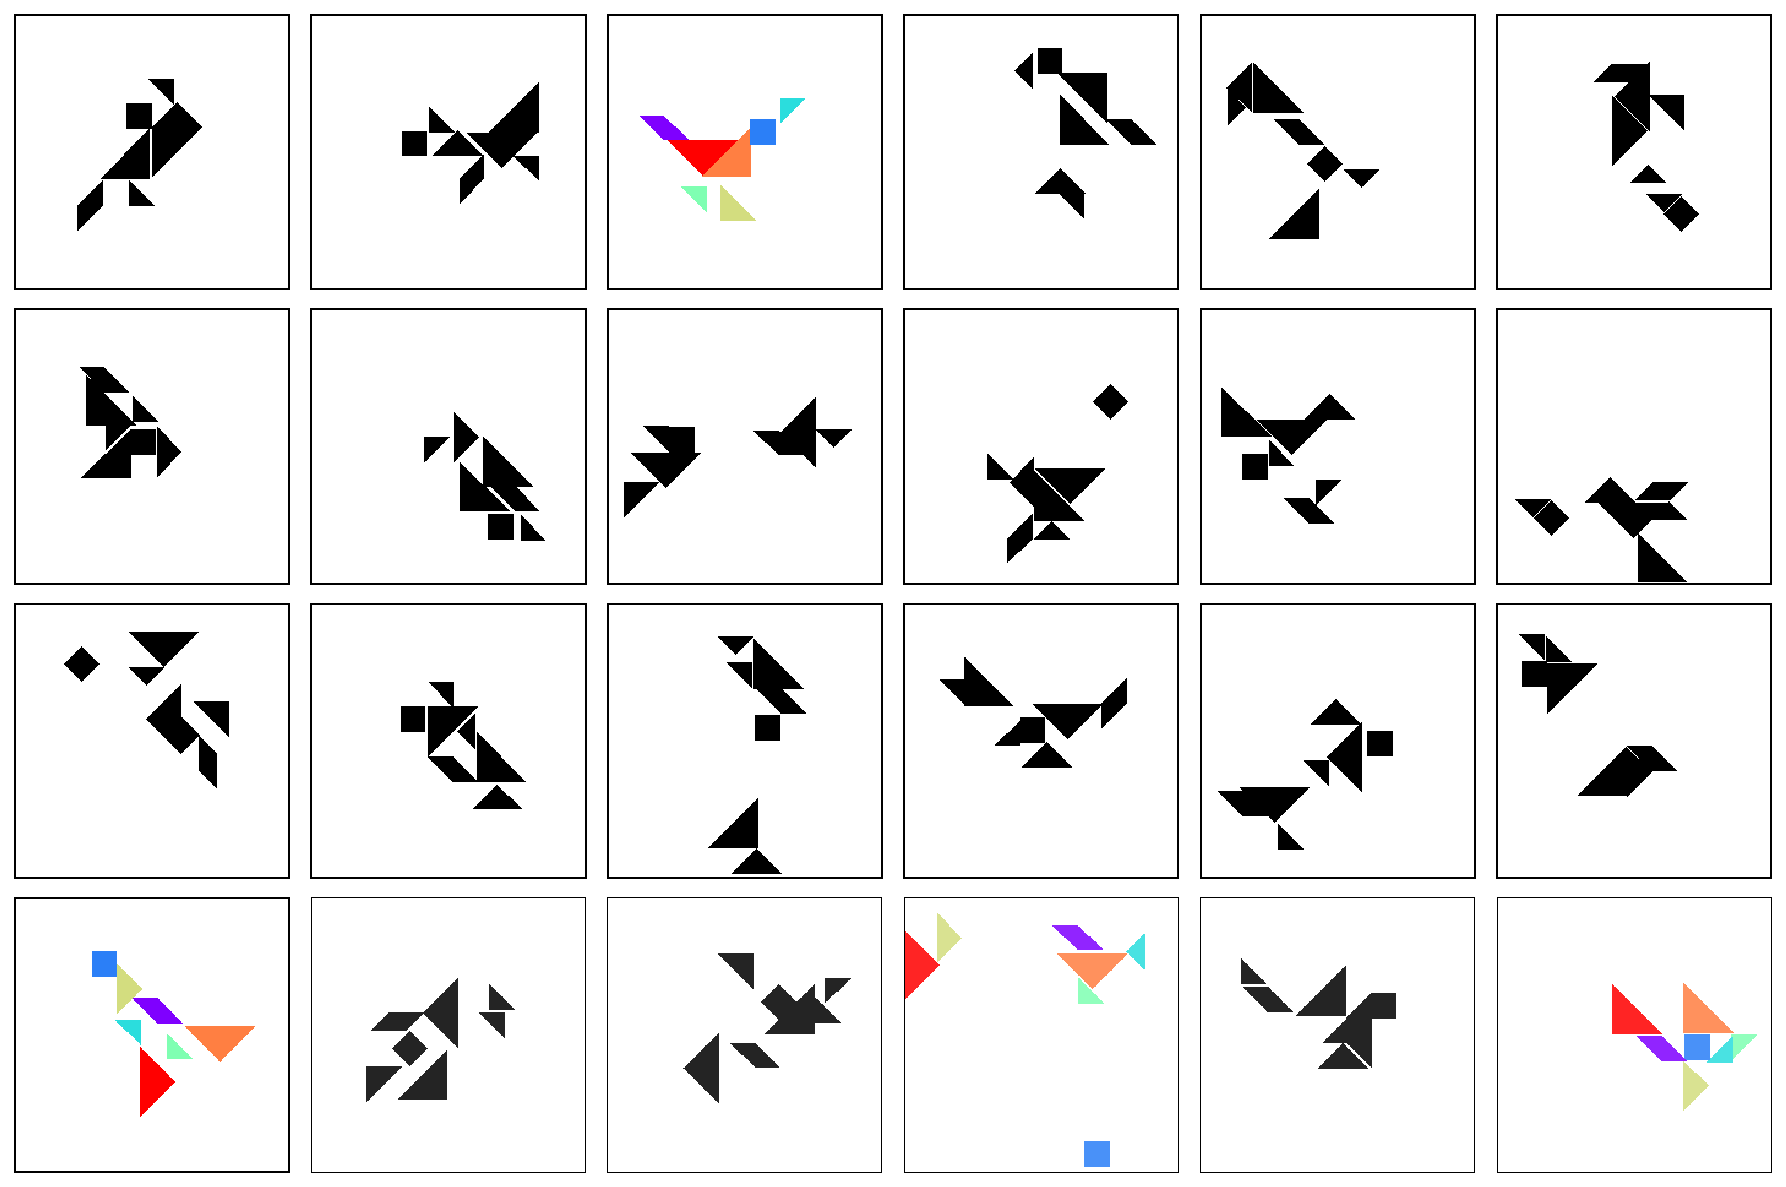
\includegraphics[width=\textwidth]{images/curation_bird.pdf}
    \caption{Birds on Tangram.}
    \label{fig:curation_bird}
\end{figure}

% curation_teapot.pdf
% curation_teapot_.pdf
% curation_teapot_all.pdf
\begin{figure}[H]
    \centering
    % 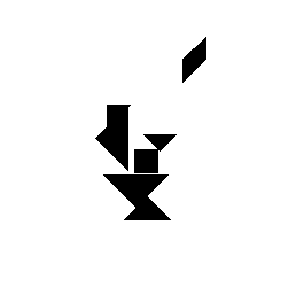
\includegraphics[width=\textwidth]{images/curation_teapot.pdf}
    % 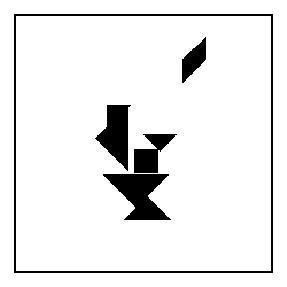
\includegraphics[width=\textwidth]{images/curation_teapot_.pdf}
    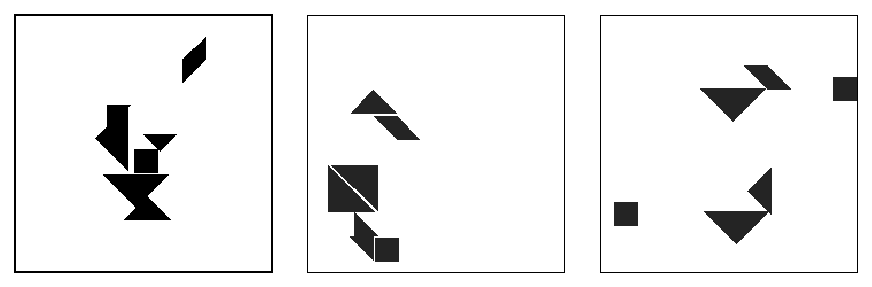
\includegraphics[width=0.5\textwidth]{images/curation_teapot_all.pdf}
    \caption{Teapots on Tangram.}
    \label{fig:curation_teapot}
\end{figure}

% curation_chair.pdf
% curation_chair_cropped.pdf
\begin{figure}[H]
    \centering
    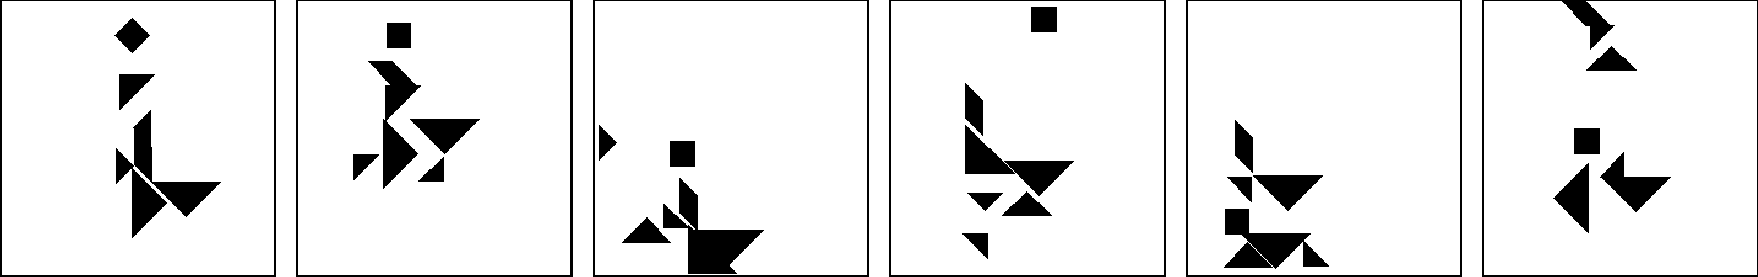
\includegraphics[width=\textwidth]{images/curation_chair_cropped.pdf}
    \caption{Chairs on Tangram.}
    \label{fig:curation_chair}
\end{figure}

% curation_heart.pdf
% curation_heart_all.pdf
\begin{figure}[H]
    \centering
    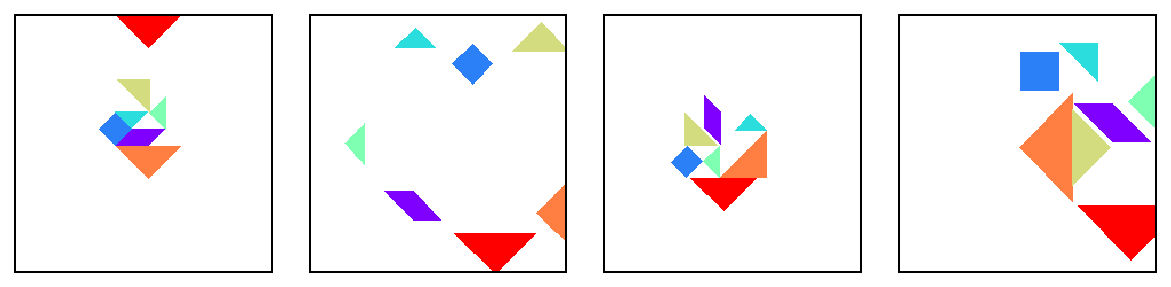
\includegraphics[width=0.66\textwidth]{images/curation_heart.pdf}
    % 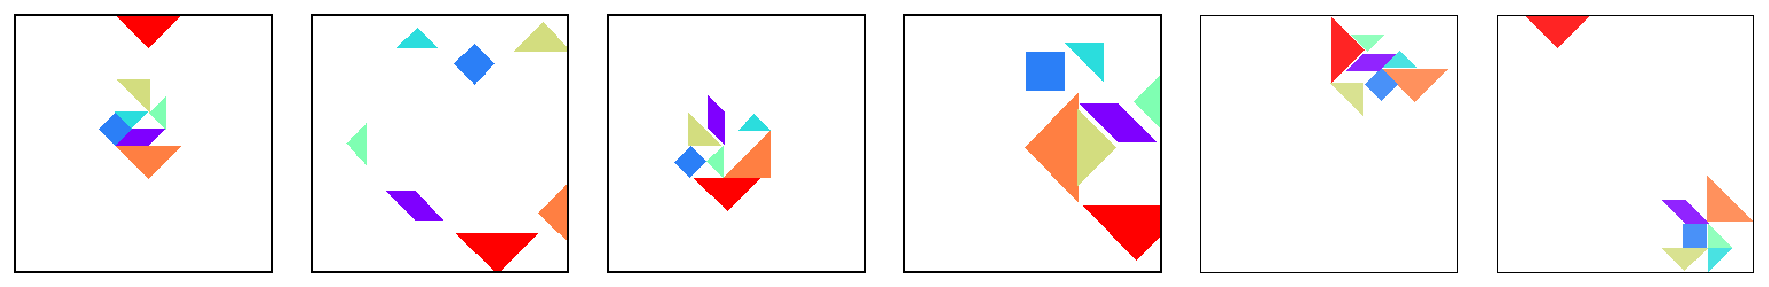
\includegraphics[width=0.66\textwidth]{images/curation_heart_all.pdf}
    \caption{Hearts on Tangram.}
    \label{fig:curation_heart}
\end{figure}

% curation_letters.pdf
\begin{figure}[H]
    \centering
    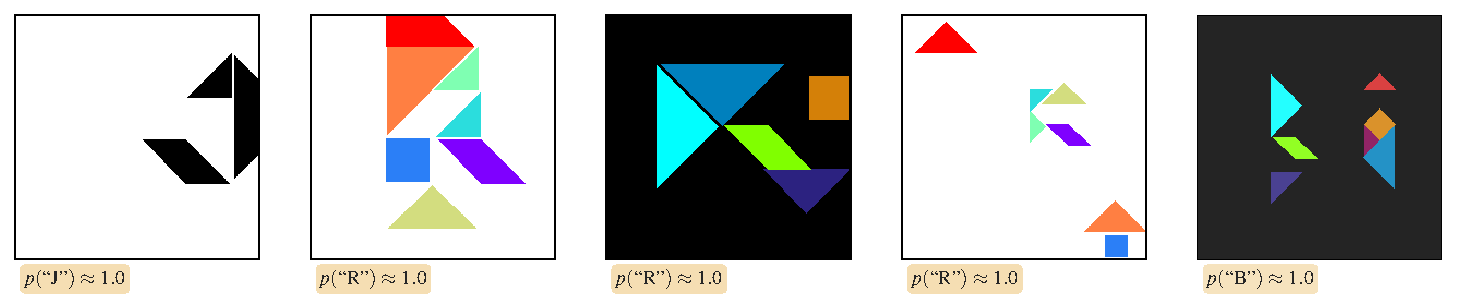
\includegraphics[width=0.824\textwidth]{images/curation_letters.pdf}
    \caption{Letters on Tangram.}
    \label{fig:curation_letters}
\end{figure}

% % sgw_reruns.pdf
% \begin{figure}[H]
%     \centering
%     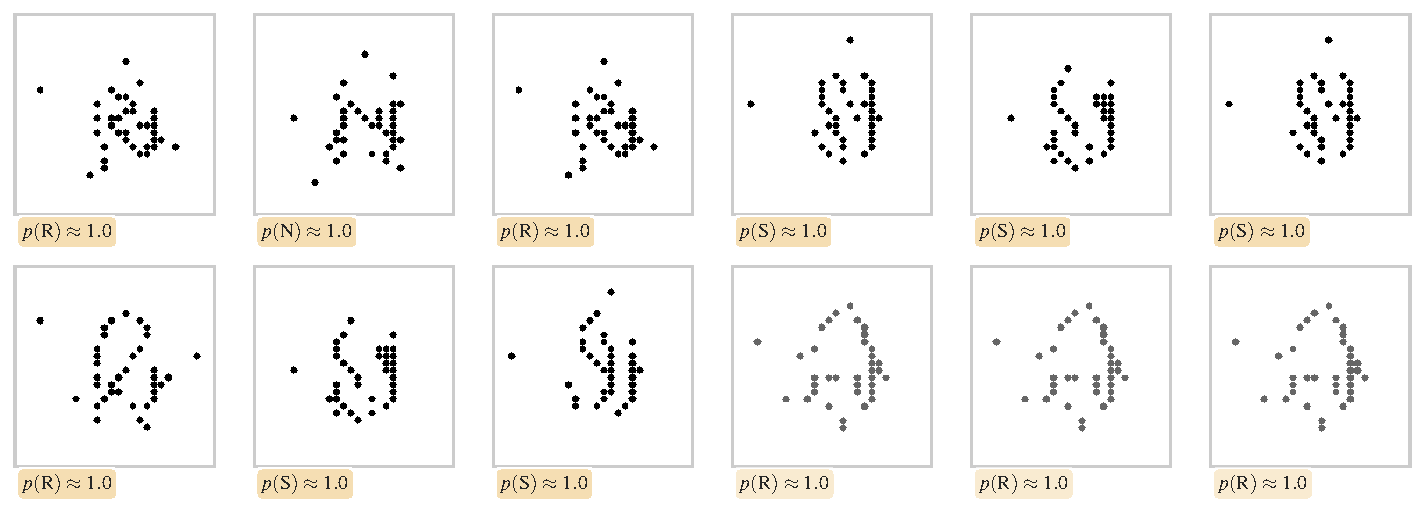
\includegraphics[width=\textwidth]{images/sgw_reruns.pdf}
%     \caption{Letters on ShapeGridWorld.}
%     \label{fig:sgw-trajectories}
% \end{figure}

% curation_animals.pdf
% curation_faces_a.pdf
% curation_faces_all.pdf
\begin{figure}[H]
    \centering
    % 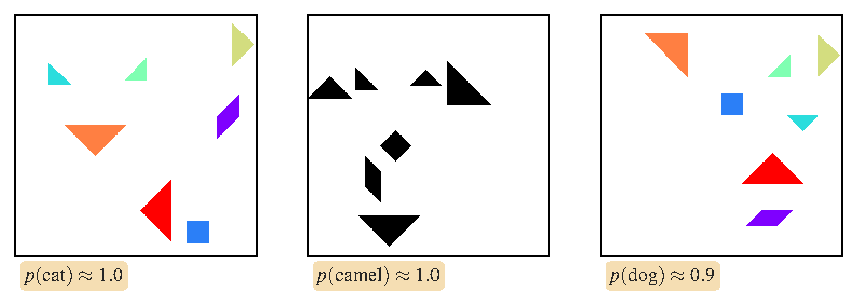
\includegraphics[width=\textwidth]{images/curation_animals.pdf}
    % 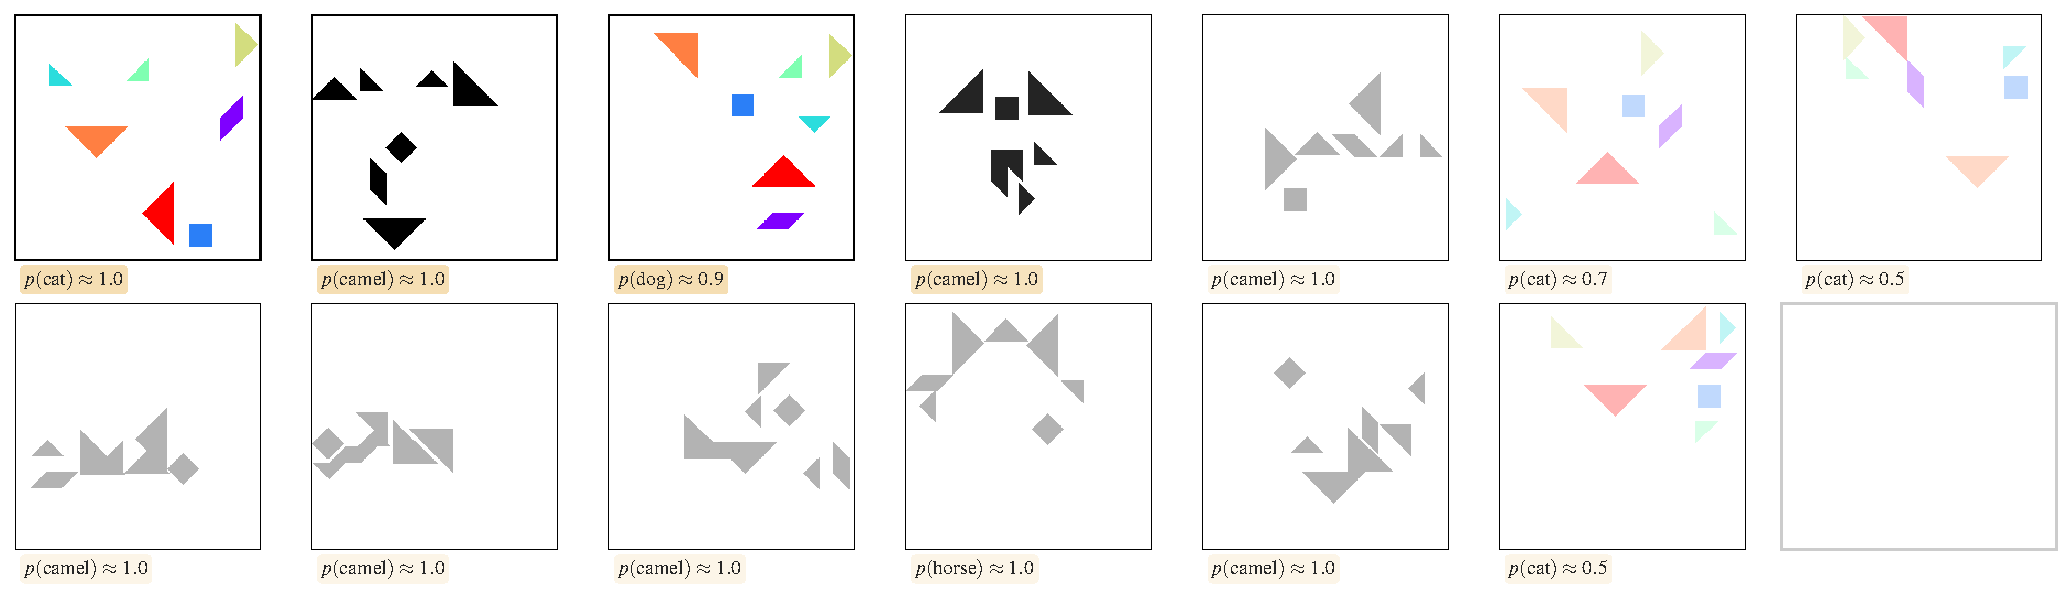
\includegraphics[width=\textwidth]{images/curation_faces_a.pdf}
    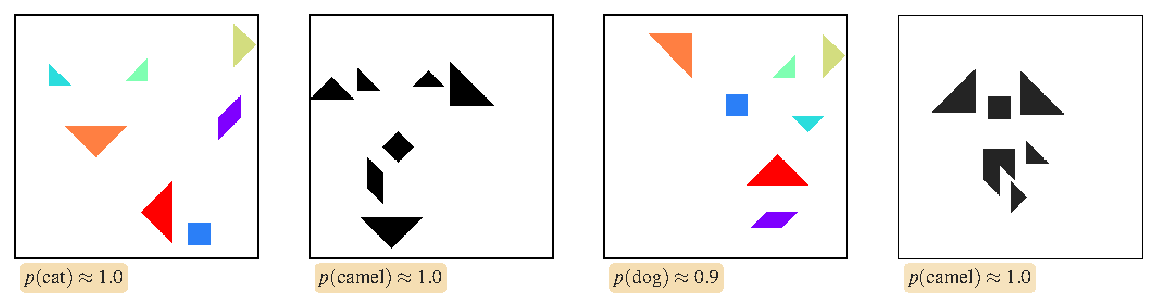
\includegraphics[width=0.66\textwidth]{images/curation_faces_all.pdf}
    \caption{Animals on Tangram.}
    \label{fig:curation_animals}
\end{figure}

% curation_shirt_all.pdf
\begin{figure}[H]
    \centering
    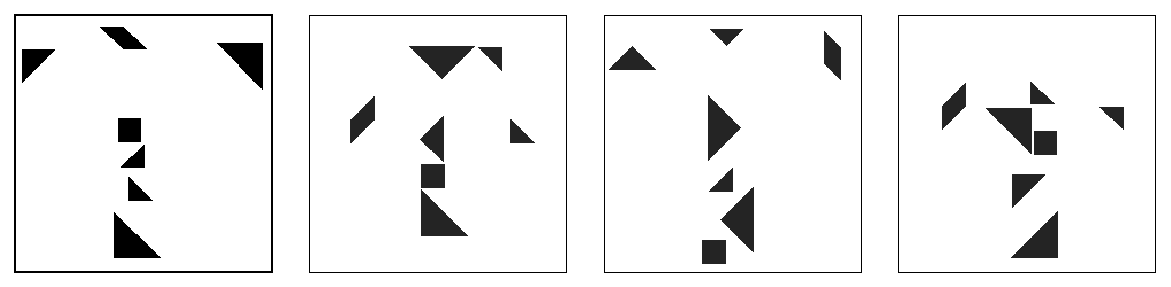
\includegraphics[width=0.66\textwidth]{images/curation_shirt_all.pdf}
    \caption{Shirts on Tangram.}
    \label{fig:curation_shirt_all}
\end{figure}

% curation_house.pdf
\begin{figure}[H]
    \centering
    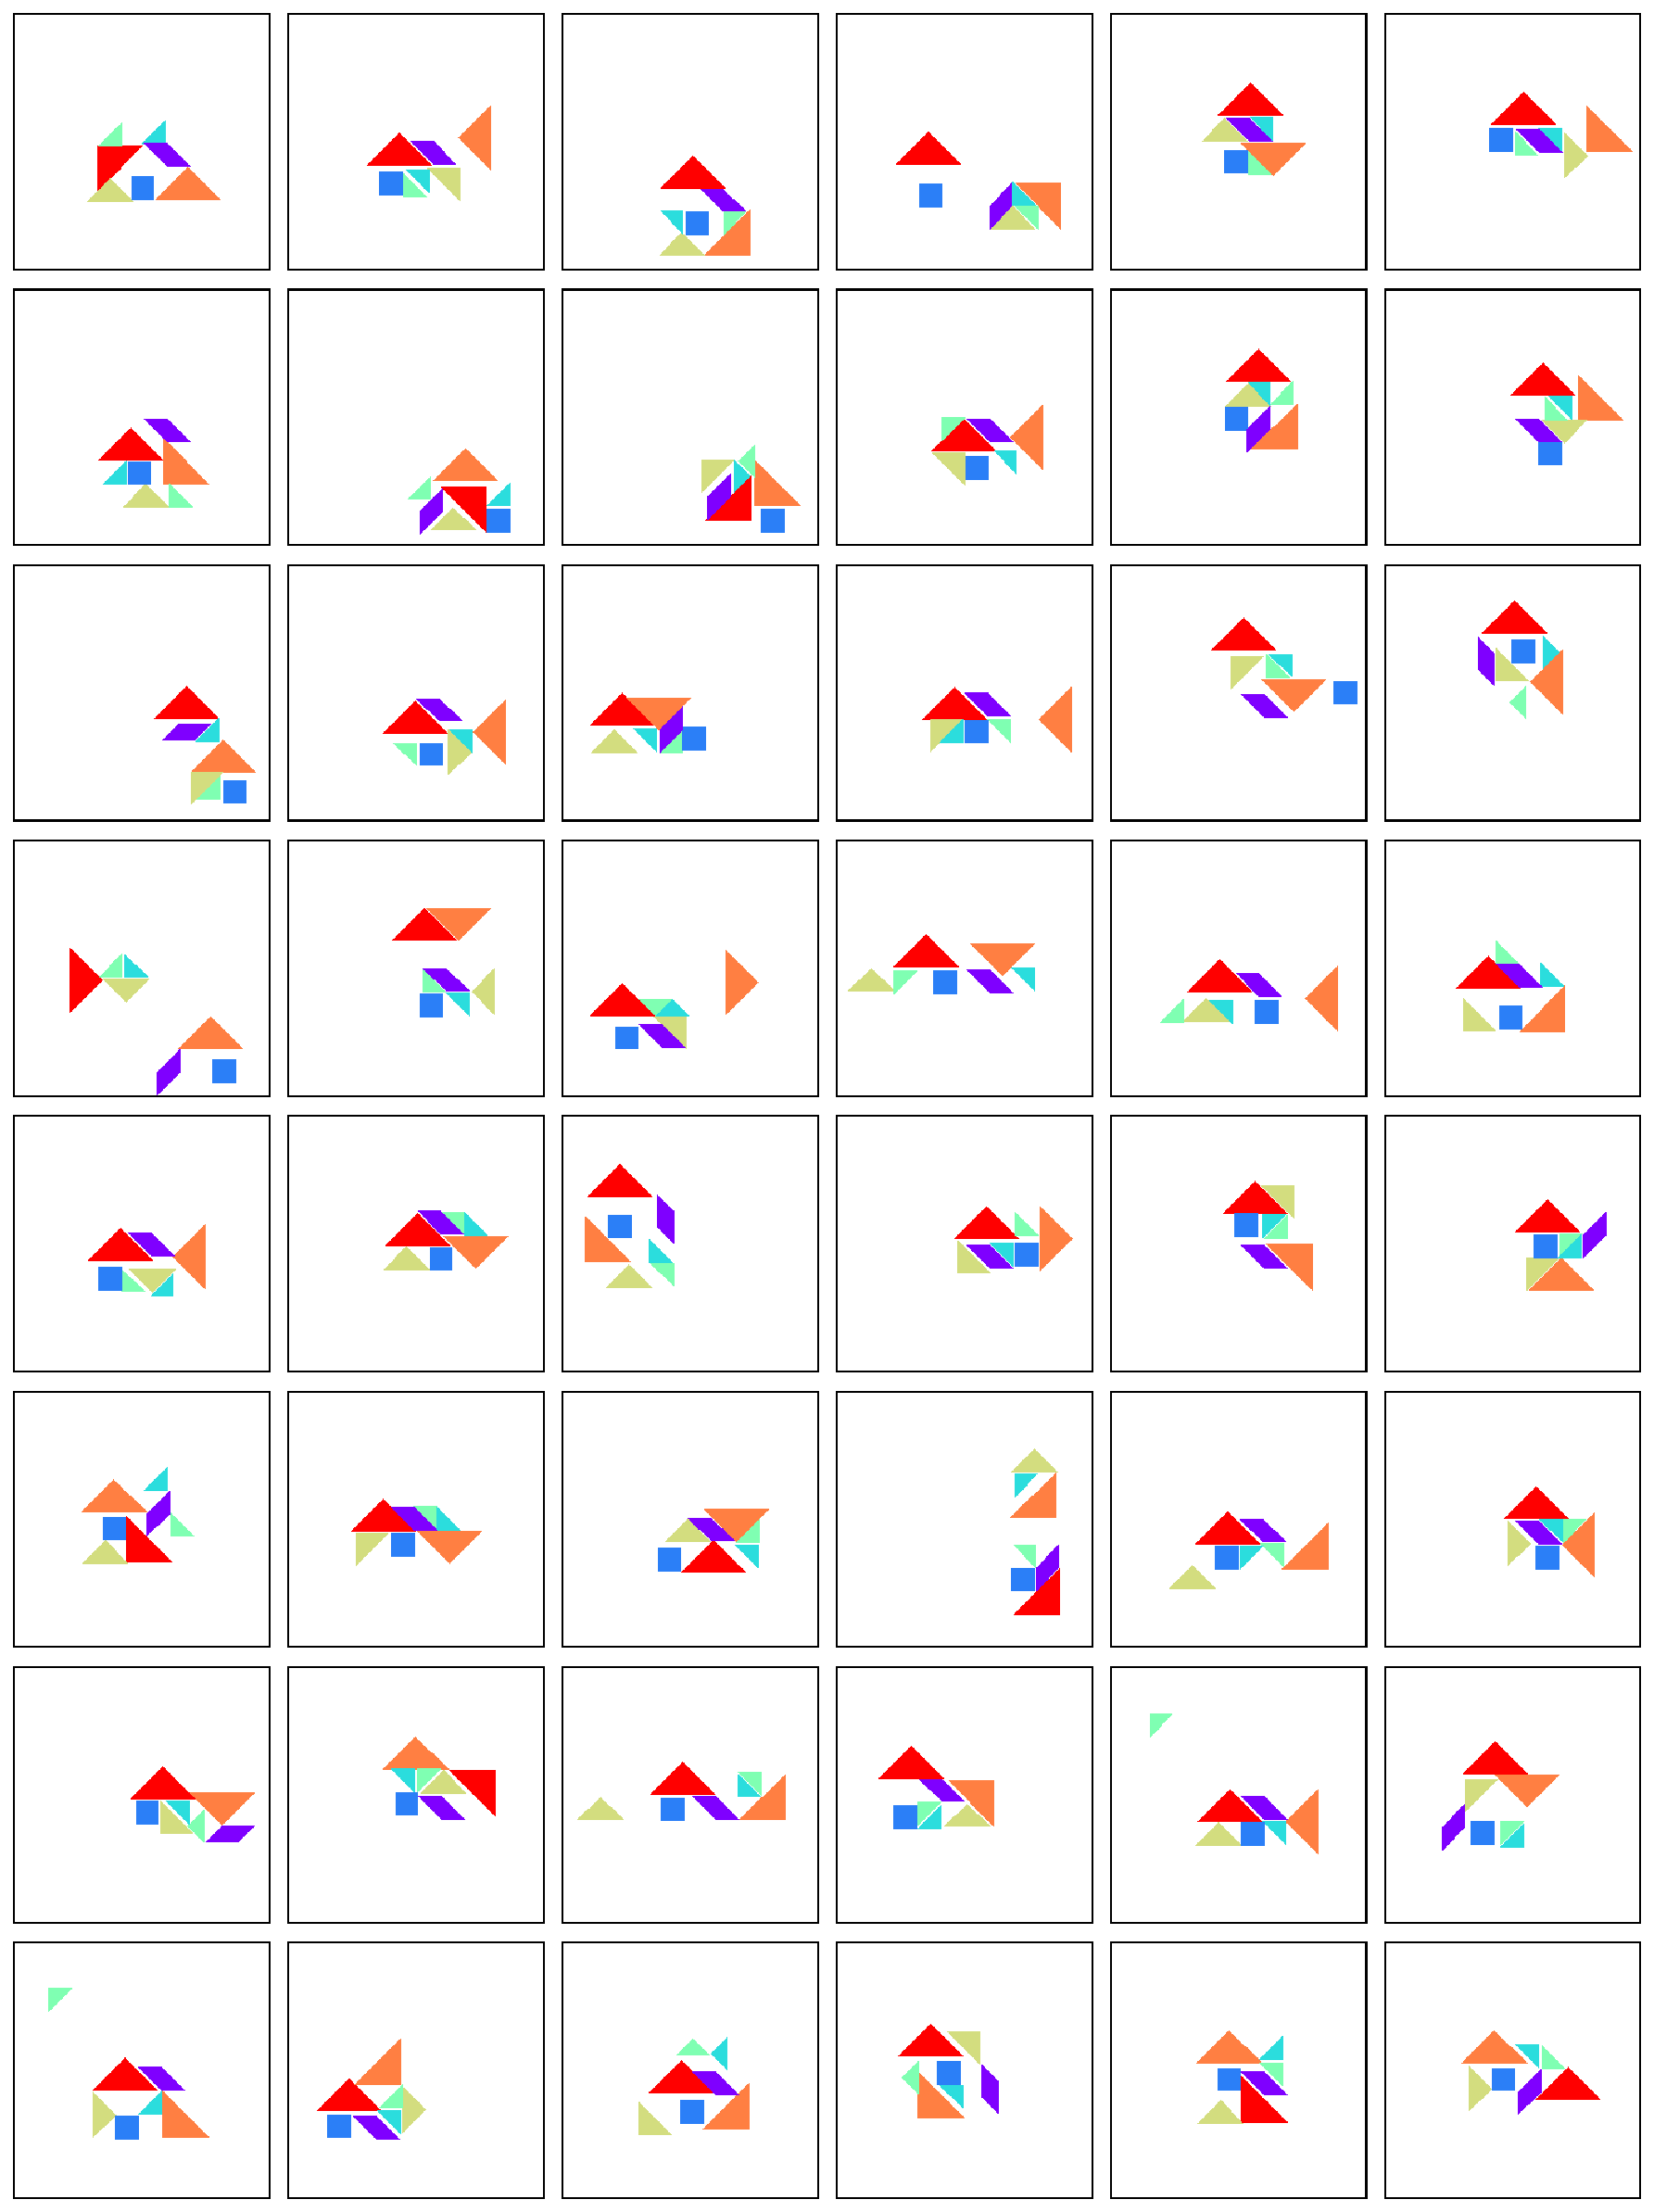
\includegraphics[width=\textwidth]{images/curation_house.pdf}
    \caption{Houses on Tangram.}
    \label{fig:curation_house}
\end{figure}

% curation_gun_all.pdf
% curation_sgw_objects.pdf
% curation_sgw_objects_cropped.pdf
\begin{figure}[H]
    \centering
    
\includegraphics[width=0.5\textwidth]{images/curation_gun_all.pdf}
    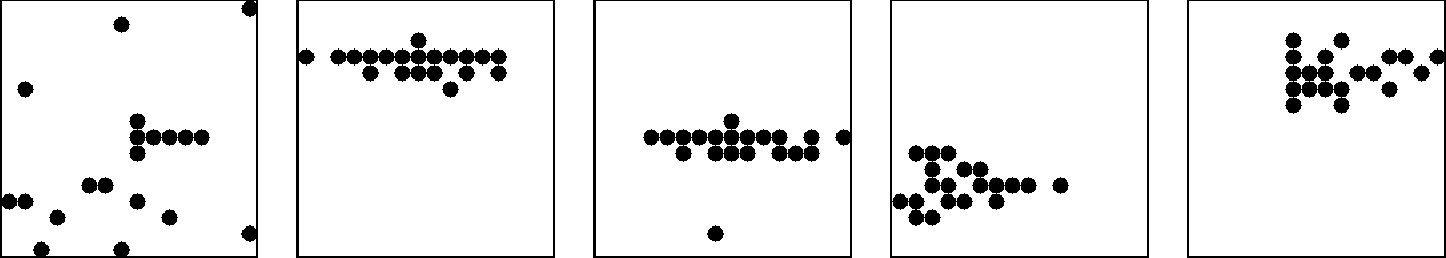
\includegraphics[width=0.824\textwidth]{images/curation_sgw_objects_cropped.pdf}
    \caption{Guns on Tangram and ShapeGridWorld.}
    \label{fig:curation_gun_all}
\end{figure}

% % curation_objects.pdf
% \begin{figure}[H]
%     \centering
%     \includegraphics[width=\textwidth]{images/curation_objects.pdf}
%     \caption{Objects on Tangram.}
%     \label{fig:curation_objects}
% \end{figure}

% curation_sgw_letters.pdf
\begin{figure}[H]
    \centering
    \includegraphics[width=\textwidth]{images/curation_sgw_letters.pdf}
    \caption{Letters on ShapeGridWorld.}
    \label{fig:curation_sgw_letters}
\end{figure}

% % curation_sgw_N.pdf
% \begin{figure}[H]
%     \centering
%     \includegraphics[width=\textwidth]{images/curation_sgw_N.pdf}
%     \caption{The letter ``N'' on ShapeGridWorld.}
%     \label{fig:curation_sgw_N}
% \end{figure}

% curation_sgw_numbers.pdf
\begin{figure}[H]
    \centering
    \includegraphics[width=\textwidth]{images/curation_sgw_numbers.pdf}
    \caption{Numbers on ShapeGridWorld.}
    \label{fig:curation_sgw_numbers}
\end{figure}

% % curation_sgw_objects.pdf
% \begin{figure}[H]
%     \centering
%     \includegraphics[width=\textwidth]{images/curation_sgw_objects.pdf}
%     \caption{Objects on ShapeGridWorld.}
%     \label{fig:curation_sgw_objects}
% \end{figure}

% \newpage
% % curation_tree.pdf
% % curation_tree_.pdf
% \begin{figure}[h]
%     \centering
%     \includegraphics[width=\textwidth]{images/curation_tree.pdf}
%     % \includegraphics[width=\textwidth]{images/curation_tree_.pdf}
%     % \caption{Trees on Tangram.}
%     \label{fig:curation_tree}
% \end{figure}

% curation_fish.pdf
% curation_fish_.pdf
% curation_fish_2.pdf
\begin{figure}[H]
    \centering
    \includegraphics[width=\textwidth]{images/curation_fish.pdf}
    % \includegraphics[width=\textwidth]{images/curation_fish_.pdf}
    % \includegraphics[width=\textwidth]{images/curation_fish_2.pdf}
    \caption{Fishes on Tangram.}
    \label{fig:curation_fish}
\end{figure}

\addtocontents{toc}{\protect\setcounter{tocdepth}{2}}
